
\chapter{Polytopes for time-efficient and reactive Cartesian space trajectory planning}
\label{ch:topca}


Previous chapters, \Cref{ch:phisical_ability_metrics}, showed that polytopes are an accurate characterisation of physical abilities for both robots and humans, as well as that the efficient polytope algebra tools potentially open doors for their use in real-time applications, \Cref{ch:transformin_polytopes}. 

One such application is showcased in \Cref{ch:physical_interaction}, demonstrating the potential of using real-time evaluation of human's and robot's physical ability polytopes in the context of the human-robot physical interaction. The chapter showed that their polytopes can be used for creating more flexible robot control strategies that adapt to the changing physical abilities of both humans and robots. A different polytope application scenario is brought in \Cref{ch:hfr}. This chapter proposes using the physical ability polytopes as a visual communication tool, providing insight to the operators about the robot's current states and its current physical abilities in real-time.




% \todos{
% \begin{itemize}
%     \item previous chapters showed how polytopes are precise characterisation of robot's physical abilities
%     \item and that we can calculate them in real-time
%     \item then chapters also show that the polytopes can be used enhancing human-robot physical collaboration by creating more flexible robot control strategies that adapt to the changing capacities of both humans and robots
%     \item also that polytopes have potential as a communication tools giving insight to the operators about the robot's current stats
% \end{itemize}
% }

% \todos{
% \begin{itemize}
%     \item motivate why is it important
% \end{itemize}
% }



This chapter brings the application of the polytope representation of robot's movement capacity (its physical ability to generate movement: velocities, accelerations, etc.) for efficient and reactive planning of robot's trajectories in \gls{cs}. 
As discussed in \Cref{ch:robot_metrics}, robot's \gls{cs} movement capacity is robot's state dependent and can change significantly while executing different trajectories. 

Leveraging the efficient tools form polytope algebra, this chapter proposes a new trajectory planning approach consisting in evaluating the robot's movement capacity in real-time and using it to adapt the planned trajectory to account for its changes. By re-planning in each step of the trajectory execution, the proposed approach is able to fully exploit robot's constantly changing movement capacity and at the same time be reactive to the potential changes in the trajectory itself, induced by the robot's environment. 
These properties are particularly interesting in the human-robot collaboration context, as the collaborative robots are often limited in performance, relying on the efficient use of their abilities, and working in human environments which is commonly unstructured and highly dynamical. 


The motivation for the proposed approach is described in \Cref{ch:topca_motivation}, followed by \Cref{ch:problem_statement}, which brings the intuition about the difficulties of planning robot's trajectories in \gls{cs}. The efficient method for evaluating robot's \gls{cs} movement capacity is described in \Cref{ch:capacity}, while the proposed real-time re-planning approach is introduces in \Cref{ch:tap}. 

The performance of the proposed planning method is compared against the state-of-the-art trajectory planning methods in \Cref{ch:comp_study}. And \Cref{ch:experiment_mockup} brings an applicative experiment of the proposed method in the context of collaborative waste sorting.

\section{Motivation: Time-optimal and reactive trajectories}
\label{ch:topca_motivation}
The field of collaborative robotics has seen a unprecedented growth in recent years with the development of safer and cheaper robots with promising applications in industry, research, and even everyday life \cite{ajoudani2018progress}. However, as the complexity of the environments in which these robots operate increases, planning for robot trajectories becomes a significant challenge.  The robots need to adapt to changing environmental conditions and tasks, as well as the presence of humans. 
At the same time, in order to be safe, collaborative robots tend to be smaller and relatively limited in performance compared to more traditional industrial robots \cite{smu}. Therefore, it is becoming increasingly important to utilise the physical abilities of these robots fully in order for their applications to become viable, rather than investing in larger, more expensive industrial robots. 

%In addition, standard \textit{a priori} metrics of robot's physical abilities which underestimate them significantly do not scale well to these smaller robots, and new more precise and real-time capable solutions are needed to exploit their full potential.

When it comes to planning robot motions, the most common approach is to decouple path and trajectory planning \cite{Pardo1996}. First, the robot's geometric path is found, accomplishing certain task and potentially avoiding the obstacles in the environment. Then the optimal sequence of movements along this path is calculated in order to optimise certain criteria, the most common ones used in the literature being minimum energy, minimum jerk and minimum execution time. Among these criteria, the one that aims to exploit full robot's movement capacity corresponds to the minimum time criteria, resulting in time-optimal (or minimum time) trajectories \cite{Gasparetto2012}. 

Traditional time-optimal trajectory planning techniques, developed for industrial robots, find trajectories with the highest possible speeds, within robot's and task constraints, along predefined paths. These methods are often defined in robot's \gls{js} calculating the necessary optimal motions of each one of the robot's joints. Time-optimal algorithms, such as ones proposed \citet{bobrow1985time} and recently by \citet{Pham2018}, assume full in advance knowledge about both robot's path and the the environment. However in collaborative scenarios, environment is often dynamic and conditions may change rapidly, requiring real-time changes in the trajectory and the task. To account for these changes the trajectory needs to be adapted in real-time, however time-optimal approaches have long execution times due to their computational complexity, making such implementations unpractical. 


\begin{figure}[!t]
    \centering
    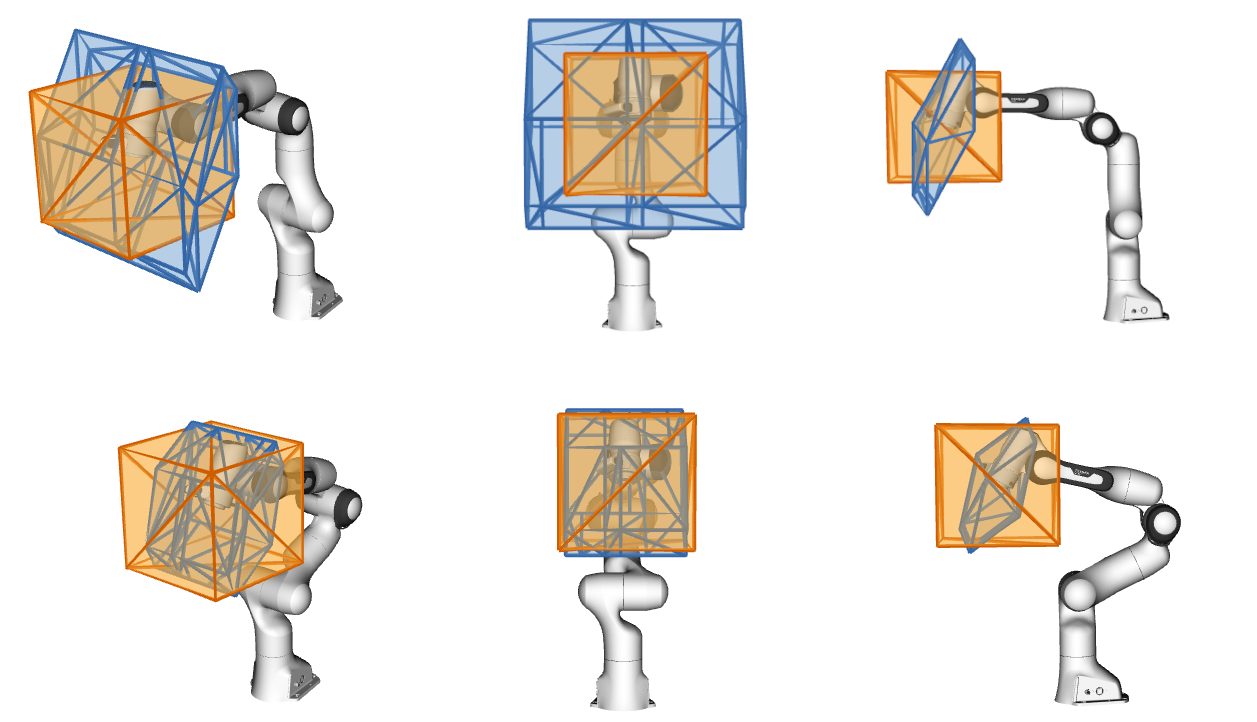
\includegraphics[width=0.8\linewidth]{Papers/imgs/comp_poly2.png}
    \caption{End-effector linear velocity limits as computed using the fixed \gls{cs} limits provided by the manufacturer (orange) and using an estimation based on the \gls{js} velocity limits and the current configuration of the robot (blue) (scale: 1 m.s$^{-1}$/ 10 cm). The true robot's velocity capacity are in some directions higher and in the others significantly lower than the manufacturer's limits, depending on the configuration.}
    \label{fig:comp_cube_poly}
\end{figure}



On the other end of the spectrum, the real-time capable trajectory planning approaches often abstract the robot as a generator of ideal movements without accounting for its true capacity. These methods are often defined in robot's task space, the space of robot's \gls{cs} positions and orientations. With this simplification, they have short execution times and can quickly adapt to any changes in the robot's path, environment or the task itself. Such algorithms, as proposed by \citet{Macfarlane2003}, \citet{haschke2008line} or \citet{Svarny2022}, are often based on S-curve trajectories \cite{FANG2019} with an appropriate order, producing smooth trajectories that respect a set of fixed velocity, acceleration, jerk and sometimes even snap (jerk derivative) limits enforced by the task itself and robot's movement capacity that is assumed to be constant \cite{modernrobotics}. However, robot's \gls{cs} movement capacity is not constant and can vary significantly during the trajectory execution, therefore such approaches are not capable of fully exploiting the robot's capacity, resulting in trajectories that might underestimate or sometimes even overestimate its movement capacity. \Cref{fig:comp_cube_poly} shows an example of this effect on a Franka Emika Panda collaborative robot.


To bridge this gap, several approaches were proposed recently, aiming to exploit full robot's movement capacity while allowing for reactive adaptations online. These methods often decouple time-optimality and reactivity problems and frequently involve varying degrees of robot model simplification.
For instance, \citet{Palleschi2021} proposed a decoupling method that plans for time-optimal robot motions while guaranteeing human safety. The approach consists in offline pre-calculation of the time-optimal trajectory that exports full robot's movement capacity, while the reactivity is ensured online using the reactive re-planning approach. 
A different decoupling approach that uses \gls{dmp} is proposed by \citet{dmp2014}. Their method calculates the \gls{dmp} models of the time-optimal point-to-point trajectories of the robot in-advance, trying to exploit its full movement capacity. Then these \gls{dmp} based trajectories are exploited in real-time to adapt to changing targets. However, even though the offline trajectories calculated by these decoupled methods are time-optimal, their real-time adaptations might lose this property. 
In order to avoid the decoupling, \citet{ZHANG2020} proposed a real-time method for time-optimal trajectory planning based on simplifying the robot's model. The approach uses machine learning to learn the simplified robot's dynamical model offline. The simplified model reduces the computational complexity of the time-optimal planning and allows for real-time reactive re-planning. However, this method requires a substantial degree of in-advance computation in order to work properly. 


Optimal control methods like \gls{mpc}~\cite{Kouvaritakis2016} offer a promising avenue for generating reactive and time-optimal trajectories in real-time. \gls{mpc} approaches determine the optimal action to be executed by the robot, given its current state and predictions of its future states, obtained using the robot's model. \gls{mpc} updates its prediction of the robot's future states in each step of the trajectory execution, taking in account the changes in robot's current state and its environment. Therefore, they are can account for the evolving movement capacity of a robot and react to the changes in its environment \cite{torresalberto2022}\cite{Eckhoff2022}. However, their implementation remains complex and challenging due to their reliance on nonlinear optimisation techniques \cite{kelff2021,Massaro2023}.

Hence, this chapter proposes a step in this direction, proposing a trajectory planning approach capable of producing time-efficient and reactive trajectories by re-planning in real-time.  
The proposed approach evaluates the robot's \gls{cs} movement capacity in real-time, using the efficient tools from polytope algebra, and re-plans the time-optimal trajectory in each time-step. The time-optimal planning is based on \gls{tap} \cite{modernrobotics} planning, which  computational efficiency enables real-time execution. 
By evaluating robot's \gls{cs} movement capacity and re-planning the time-optimal trajectory in each step of the trajectory execution, the approach is capable of adapting to the changes in robot's movement capacity without requiring any in advance computation. 
Additionally, the real-time re-planning enables reacting to potential changes in the robot's trajectory induced by its environment, making it well-suited for dynamic environments where conditions change rapidly such as human-robot collaboration. 

Experimental results, described in \Cref{ch:comp_study}, demonstrate the effectiveness of the proposed approach on a Franka Emika Panda collaborative robot. The proposed method is compared against the state-of-the art offline time-optimal method TOPP-RA \cite{Pham2018}, where the results show that the proposed algorithm generates the trajectories that have comparable execution time (even shorter in some cases) than offline method.
The method is furthermore compared to the standard reactive approach based on \gls{tap} planning with fixed \gls{cs} movement capacity given by the manufacturer.  The analysis confirms that the proposed method achieves faster and more precise trajectories than the standard reactive approach with fixed capacity assumption. 

Finally the reactivity of the proposed approach is demonstrated in the mock-up experiment in the context of collaborative waste sorting, described in \Cref{ch:experiment_mockup}. In this experiment the proposed planning method was used to generate time-efficient and adaptable robot's trajectories in order to pick the waste items introduced by the operator and place them in the appropriate sorting bins.

The intuition about robot's movement capacity aware trajectory planning in \gls{cs} is given in \Cref{ch:problem_statement}. 
The description of the efficient method for robot's \gls{cs} movement capacity evaluation is described in \Cref{ch:capacity}. 
Then, \Cref{ch:tap} gives an overview of the Cartesian space \gls{tap} planning and the description of the real-time planning strategy. 
The experimental setup for assessing the performance of the proposed method on a Franka Emika Panda collaborative robot is given in \Cref{ch:setup}. 




\section{Problem statement: Capacity aware trajectory planning}\label{ch:problem_statement}

Time-optimal trajectory planning consists in finding the robot's movements with the highest possible speeds, within robot's and task constraints, along predefined paths. 
Therefore it requires a thorough understanding of the robot's movement (ex. velocity, acceleration, jerk) capacity along the specified path. 
%As dissussed  ability to move along the path is highly dependant on its kinematics, dynamics and joint actuation capabilities. 

Robot's actuation capabilities are usually expressed in the $n$ dimensional \gls{js}. 
Where, for each one of $n$ joint actuators, the limits are specified by manufacturers in a form of independent min-max ranges of different joint variables. 
As opposed to the robot's actuator limits, robot's path is often defined in the task space, often $m=3$ dimensional space of \gls{cs} positions or $m=6$ if orientations are specified as well. 
In the context of this chapter robot's paths are considered to be \gls{cs} point-to-point straight line path from one pose $X_a$ to another $X_b$ (for example expressed as an homogeneous transform matrix in $SE(3)$). \gls{cs} straight line paths are commonly used as they represent the shortest paths in the \gls{cs} between the two \gls{cs} positions, and in the context of human-robot interaction they have shown to produce predictable robot's motions for the operators \cite{Dragan2013Legibility}. Additionally, they can be used to construct more complex paths by approximating them with a set of straight line segments.


Traditional approaches to the time-optimal trajectory planning consist in transforming the path to \gls{js}, where they find the fastest movements of the robot's joints following the path and respecting the actuator limits.
This approach is convenient because the robot's movement capacity is \gls{js} is constant and each joint limit is specified with an independent min-max range. 
However, the main limitation of this approach is that \gls{js} is usually higher dimensional than \gls{cs} ($n>m$), making the mapping between the \gls{cs} and \gls{js} not unique. In practice this means that there are multiple \gls{js} paths that accomplish the same \gls{cs} path. Each one of these \gls{js} paths has different properties which makes finding the optimal \gls{js} path a challenging problem of its own. Additionally, having chosen an appropriate \gls{js} path, the robot's redundant degrees of freedom are fixed even though they do not participate in movement generation, preventing it from executing other tasks and further limiting this approach.

Complementary approach consists in transforming the robot’s joint actuator limits to the \gls{cs} and planning the time-optimal trajectory in \gls{cs} directly.
Such method results in the \gls{cs} trajectory which respects all the robot's actuator limits without explicitly choosing the \gls{js} path. 
As discussed in \Cref{ch:phisical_ability_metrics}, once the robot's actuator limits are transformed to \gls{cs}, they form the polytopes of robot's \gls{cs} movement capacity.
The robot's movement polytopes are highly dependant on its state and can evolve significantly during the trajectory execution. 
Therefore, changing robot's \gls{cs} movement capacity presents one of the main challenges of time-optimal trajectory planning in \gls{cs}. 
\Cref{fig:motiv_topca} illustrates robot's changing \gls{cs} velocity capacity along the trajectory for two different \gls{js} paths executing the same \gls{cs} path. 

\begin{figure}[!t]
    \centering 
    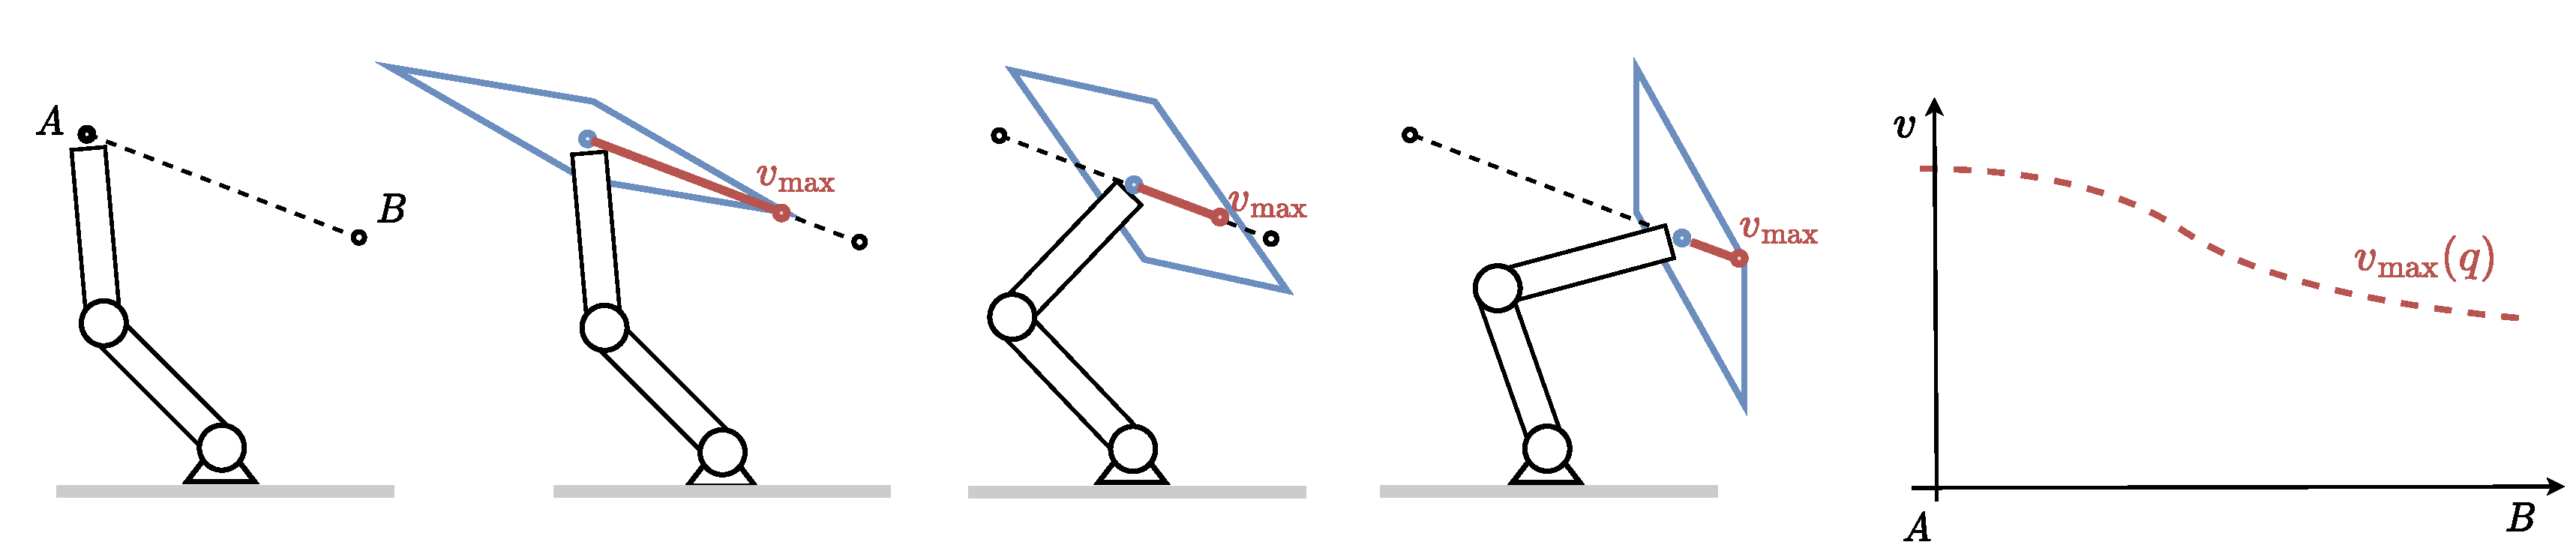
\includegraphics[width=\linewidth]{Papers/imgs/motivation_topca.pdf}
    \caption{The figure illustrates the robot's \gls{cs} linear velocity capacity evolution while following a \gls{cs} straight line path, from point A to B, using two different \gls{js} paths (up and down). The robot's \gls{cs} velocity capacity polytope is shown in blue, while its capacity to generate velocity in the path direction is shown in red. The path is shown in black dashed lines. The graph on the right shows the evolution of the robot's velocity capacity in the path direction while executing the trajectory. The figure shows that the robot's movement capacity in the path direction can evolve significantly during the trajectory execution, as well as that it depends highly on the \gls{js} path taken. }
    \label{fig:motiv_topca}
\end{figure}

A common approach to simplify this issue is to consider robot's \gls{cs} movement capacity constant during the trajectory execution. For example by choosing a fixed set of limits that correspond to the worst-case robot's movement capacity along the path. 
Such approach is, by definition, not capable of fully exploiting the robot's movement capacity, underestimating considerably robot's actual abilities. Furthermore, finding the worst-case underestimation of the robot's movement capacity involves characterising all the robot's \gls{js} configurations possible for the same path, which is not always practically possible and results in long execution times. 
A more common approach, especially in the industry, is much more empirical. It involves manually finding the appropriate set of fixed \gls{cs} limits by specifying certain percentage of the robot's \gls{cs} limits predefined by the manufacturers \cite{ur3data}\cite{frankadata}. 
This tuning approach has to be repeated for each trajectory of interest in order to find a satisfactory trade-off between robot's speed and the tracking error. Manual tuning can be time consuming and, in many cases, results in sub-optimal trajectories planed without any real information about the robot's true motion capacity. 

Therefore, choosing any fixed set of \gls{cs} limits leads to either overestimation of the robot's movement capacity or its underestimation, as shown on \Cref{fig:under_over}. The overestimation can lead to planning for trajectories that are unfeasible for the robot, while underestimation leads to sub-optimal robot's trajectories, that do not exploit its full movement potential. Planning for a true time-optimal trajectory would involve accounting for the robot's changing movement abilities along the trajectory. However, as the robot's movement capacity depends on its joint states, evaluating the robot's movement capacity along the path in advance would require transforming the \gls{cs} path to \gls{js}. Such approach would lose most of the benefits of \gls{cs} trajectory planning: resulting in high computational cost, requiring making choices about the appropriate \gls{js} path and fixing the robot's redundant degrees of freedom.


\begin{figure}[!t]
    \centering 
    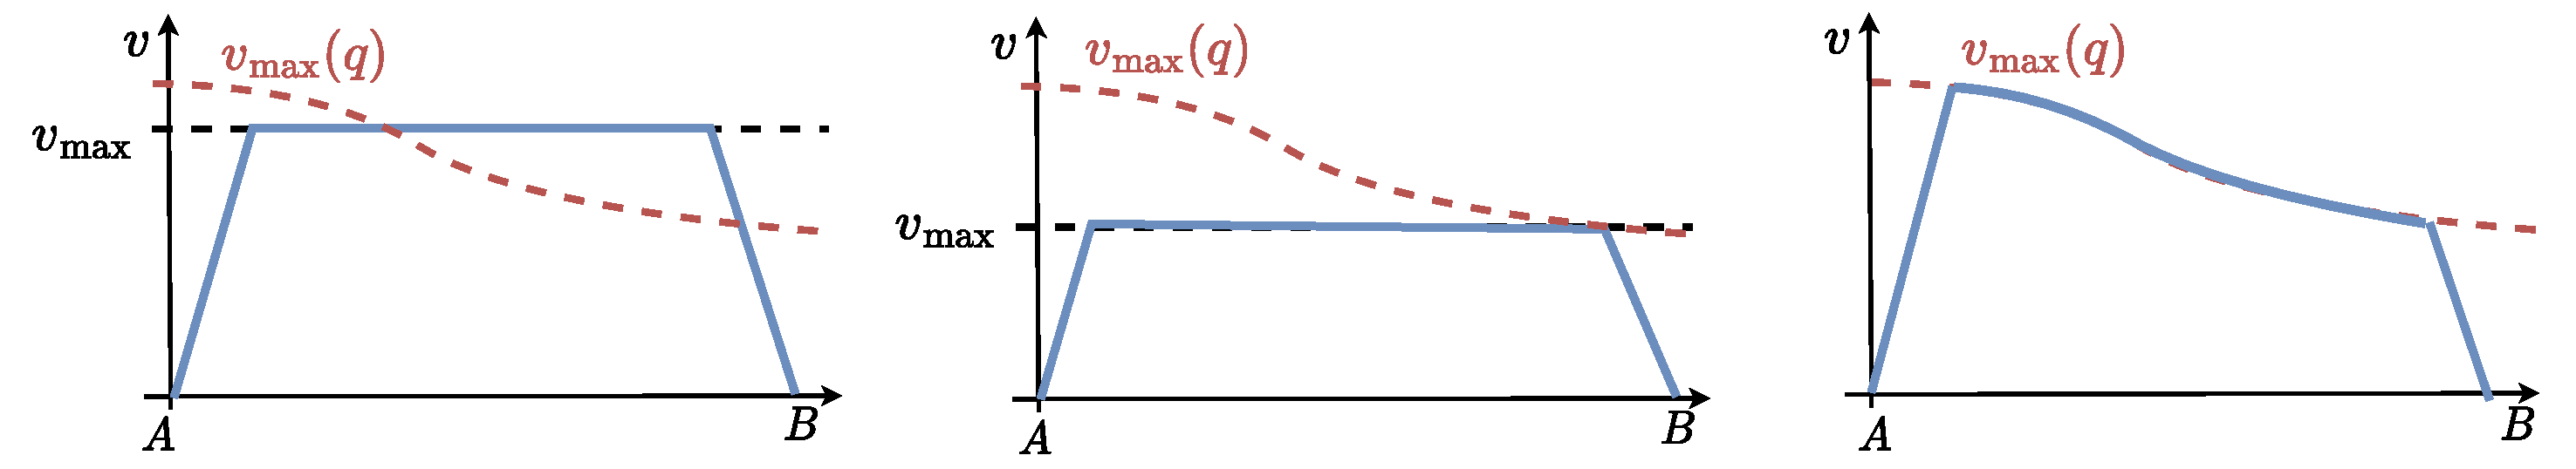
\includegraphics[width=\linewidth]{Papers/imgs/unre_over_poly.pdf}
    \caption{The figure illustrates three different strategies for planning for \gls{cs} trajectory with respect to their consideration of the robot's velocity capacity limits in the path direction. The planned trajectories are shown in blue while the robot's true velocity capacity when executing the trajectory is shown in red dashed lines. Figures on the left  and in the middle represent the planning methods which assume fixed velocity capacity during the trajectory execution (black dashed line). Strategy on the left, due to the robot's changing capacity, at the beginning of the trajectory underestimates robot's ability and towards the end overestimates robot's abilities, resulting in infeasible trajectory. Strategy in the middle uses the worst-case velocity capacity on the path as its limit, resulting in feasible trajectory however significantly underestimating robot's abilities. Strategy on the right shows an example of a true time-optimal trajectory exploiting fully robot's changing velocity capacity. }
    \label{fig:under_over}
\end{figure}

Rather than trying to account for the robot's changing movement capacity in the offline planning stage, this chapter proposes a method that calculates the robot's movement capacity in real-time and adapts the time-optimal trajectory with the updated limits in each step. 
The proposed method calculates the robot's movement capacity, in the path direction, using efficient tools from polytope algebra in real-time. \gls{tap} planning is then used to recalculate the time-optimal trajectory with the updated movement capacity is each step.
In this way, this \gls{cs} trajectory planning method is able to adapt to the robot's changing movement capacity, while not making any a priori choices about the robot's \gls{js} path. Additionally, the real-time re-planning allows the method to be reactive to the potential changes in the desired robot's path induced by the robot's environment.

The real-time method for robot's \gls{cs} movement capacity evaluation in the path direction is described in \Cref{ch:capacity}. While \Cref{ch:tap} presents the real-time \gls{tap} based trajectory re-planing method. 
\Cref{ch:comp_study} then brings a comparative study of the performance of the proposed method against the state-of-the-art \gls{js} time-optimal method TOPP-RA \cite{Pham2018}, as well as against the \gls{cs} planning approach considering fixed limits.


\section{Evaluating robot's Cartesian space movement capacity in real-time}
\label{ch:capacity}

Robot's joint actuator limits are usually given by the manufacturer as ranges of the feasible joint positions $\bm{q}\in\mathbb{R}^n$, velocity $\bm{q}\in\mathbb{R}^n$, acceleration $\dot{\bm{q}}\in\mathbb{R}^n$ and jerk $\ddot{\bm{q}}\in\mathbb{R}^n$
\begin{equation}
\begin{split}
\dddot{\bm{q}} \in [ \dddot{\bm{q}}_{min}, \dddot{\bm{q}}_{max}] , \quad\ddot{\bm{q}} \in [\ddot{\bm{q}}_{min},  \ddot{\bm{q}}_{max}],\quad
\dot{\bm{q}} \in [\dot{\bm{q}}_{min},  \dot{\bm{q}}_{max}], \quad{\bm{q}} \in [{\bm{q}}_{min},  {\bm{q}}_{max}]
\end{split}
\label{eq:topca_kin_limits}
\end{equation}

The mapping between the robot's $n$ dimensional \gls{js} and $m$ dimensional \gls{cs} velocity, acceleration and jerk for a certain fixed frame of interest (ex. end-effector frame) is nonlinear and dependant on robot's state $\{\bm{q},\dot{\bm{q}},\ddot{\bm{q}}\}$ 
\begin{equation}
\begin{split}
\dot{\bm{x}}&= J(\bm{q})\dot{\bm{q}}\\
\ddot{\bm{x}}&= J(\bm{q})\ddot{\bm{q}} + \dot{J}(\bm{q},\dot{\bm{q}})\dot{\bm{q}}\\
\dddot{\bm{x}}&= J(\bm{q})\dddot{\bm{q}} + 2\dot{J}(\bm{q},\dot{\bm{q}})\ddot{\bm{q}} + \ddot{J}(\bm{q},\dot{\bm{q}},\ddot{\bm{q}})\dot{\bm{q}}\\
 \end{split} \label{eq:topca_js_to_cs_vaj}
\end{equation}
For a certain joint configuration $\bm{q}$, the joint velocity $\dot{\bm{q}}$, acceleration $\ddot{\bm{q}}$ and jerk $\dddot{\bm{q}}$ are mapped to \gls{cs} using the Jacobian matrix $J(\bm{q})\in\mathbb{R}^{m\times n}$ and its time derivatives $\dot{J}(\bm{q},\dot{\bm{q}})\in\mathbb{R}^{m\times n}$ and  $\ddot{J}(\bm{q},\dot{\bm{q}},\ddot{\bm{q}})\in\mathbb{R}^{m\times n}$. 


\gls{js} kinematic limits (\ref{eq:topca_kin_limits}) are expressed in a form of an interval for each of the robot's $n$ joints (degrees of freedom), forming $n$ dimensional hyperrectangles. For any given robot state $\{\bm{q}_k,\dot{\bm{q}}_k,\ddot{\bm{q}}_k\}$, \gls{cs} kinematic limits can be calculated by projecting these \gls{js} $n$ dimensional hyperrectangles (\ref{eq:topca_kin_limits}) into the $m$ dimensional \gls{cs} using the expressions (\ref{eq:topca_js_to_cs_vaj}). The resulting \gls{cs} limits will have a form of convex polytopes. 

For a certain robot pose $\bm{q}_k$ the convex polytope $\mathcal{P}_v$ of achievable \gls{cs} velocities $\dot{\bm{x}}$ can be expressed as
\begin{equation}
    \mathcal{P}_v(\bm{q}_k) = \left\{ \dot{\bm{x}}\in\mathbb{R}^m ~|~~ \dot{\bm{x}}=J(\bm{q}_k)\dot{\bm{q}} + \bm{b}_v, \quad \dot{\bm{q}}\in \left[\dot{\bm{q}}_{min}, \dot{\bm{q}}_{max} \right] \right\}
    \label{eq:vel_poly}
\end{equation}
where $\bm{b}_v$ is a zero bias vector $\bm{b}_v\!=\!\bm{0}_{m\times 1}$. The convex polytopes $\mathcal{P}_a$ and $\mathcal{P}_j$ of achievable \gls{cs} acceleration $\ddot{\bm{x}}$ and jerk $\dddot{\bm{x}}$ have a form
\begin{equation}
\begin{split}
    \mathcal{P}_a(\bm{q}_k,\dot{\bm{q}}_k)  &= \left\{ \ddot{\bm{x}}\in\mathbb{R}^m ~|~~ \ddot{\bm{x}}=J(\bm{q}_k)\ddot{\bm{q}} + \bm{b}_a, \quad \ddot{\bm{q}}\in \left[\ddot{\bm{q}}_{min}, \ddot{\bm{q}}_{max} \right] \right\}\\
    \mathcal{P}_j(\bm{q}_k,\dot{\bm{q}}_k,\ddot{\bm{q}}_k) &= \left\{ \dddot{\bm{x}}\in\mathbb{R}^m ~|~~ \dddot{\bm{x}}=J(\bm{q}_k)\dddot{\bm{q}} +\bm{b}_j, \quad \dddot{\bm{q}}\in \left[\dddot{\bm{q}}_{min}, \dddot{\bm{q}}_{max} \right] \right\}
\end{split}\label{eq:jerk_acc_poly}
\end{equation}
where $\bm{b}_a$ and $\bm{b}_j$ are the bias acceleration and jerk produced by the effect of current joint velocity $\dot{\bm{q}}_k$ and acceleration $\ddot{\bm{q}}_k$ 
\begin{equation}
\begin{split}
\bm{b}_a&= \dot{J}(\bm{q}_k,\dot{\bm{q}}_k)\dot{\bm{q}}_k\\
\bm{b}_j&= 2\dot{J}(\bm{q}_k,\dot{\bm{q}}_k)\ddot{\bm{q}}_k + \ddot{J}(\bm{q}_k,\dot{\bm{q}}_k,\ddot{\bm{q}}_k)\dot{\bm{q}}_k\\
 \end{split} \label{eq:bias_terms}
\end{equation}
Additionally, as the $\bm{b}_j$ term produced by the second derivative of the Jacobian matrix $\ddot{J}\dot{\bm{q}}_k$ will produce relatively small effects on final value of $\bm{b}_j$, in the case of this work, it is neglected $\ddot{J}\dot{\bm{q}}_k \approx 0$. Finally, the achievable \gls{cs} velocity, acceleration and jerk, given current robot state $\bm{q}_k,\dot{\bm{q}}_k,\ddot{\bm{q}}_k$ can be expressed as
\begin{equation}
    \dot{\bm{x}}\in \mathcal{P}_v(\bm{q}_k), \quad \ddot{\bm{x}}\in \mathcal{P}_a(\bm{q}_k,\dot{\bm{q}}_k), \quad \dddot{\bm{x}}\in \mathcal{P}_j(\bm{q}_k,\dot{\bm{q}}_k,\ddot{\bm{q}}_k)\label{eq:limits_poly}
\end{equation}

As point-to-point \gls{cs} paths are effectively one dimensional, instead of using the complete polytope definitions (\ref{eq:vel_poly}) and (\ref{eq:jerk_acc_poly}), a more efficient solution is to use the polytopes to find the robot's movement capacity in the path direction. Since the path is one dimensional the calculated movement capacity can be expressed in a form or min-max ranges (intervals) for each one of the \gls{cs} variables. 
% In practice, most of the off-the-shelf trajectory planning algorithms is defined for min-max range shaped limits. 
The following section proposes an efficient approach to finding the projection of the \gls{cs} polytopes of robot's movement capacity in the path direction.

\subsection{Finding movement capacity in the path direction}
\label{ch:capacity_lp}

Characterising the robot's movement (velocity, acceleration and jerk) capacity in the path direction, requires finding the maximal (and minimal) values of the robot's \gls{cs} movement variable in the path direction that is still withing its movement capacity polytope. In other words, geometrically, this corresponds to finding the intersection of the polytope with the line corresponding to the path direction. Therefore, this section proposes an efficient \gls{lp} based approach for characterising this intersection.

\begin{wrapfigure}{r}{0.3\linewidth}
\vspace{-0.5cm}
    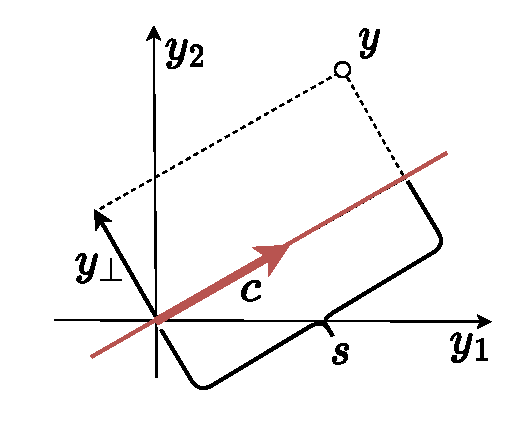
\includegraphics[width=\linewidth]{Papers/imgs/decomposiiton.pdf}
    \label{fig:decomp}
    \caption{Figure shows the projection $s$ of the \gls{cs} variable in the path direction $\bm{c}$ as well as its components $\bm{y}_{\perp}$ normal to the path.}
\end{wrapfigure}
For any point-to-point \gls{cs} path, an $m$ dimensional \gls{cs} unit vector $\bm{c}$, pointing in the direction of the path can be found. Then any \gls{cs} vector $\bm{y}\in\mathbb{R}^m$ can be projected on the path direction using the scalar product
\begin{equation}
s = \bm{c}^T\bm{y}
\label{eq:path_direction}
\end{equation}
where $s\in\mathbb{R}$ is a scalar. Analogously, the projection of the vector $\bm{y}$ on the path's complementary (orthogonal) space can be expressed using \cite[p. 431]{meyer2001Matrix}
\begin{equation}
\bm{y}_\perp = \underbrace{(I_{m\times m} - \bm{c}\bm{c}^T)}_{N}\bm{y}
\label{eq:path_orthoonal}
\end{equation}
where $\bm{y}_\perp\in\mathbb{R}^m$ is a $m$ dimensional vector containing the components of the vector $\bm{y}$ orthogonal to the path. Mathematically, the matrix $N = (I_{m\times m} - \bm{c}\bm{c}^T)$ corresponds to the projector to the null-space $\ker{\bm{c}}$ of the vector $\bm{c}$. A simple check can then be devised to verify if a certain \gls{cs} vector $\bm{y}$ is in the path direction. In order for vector $\bm{y}$ to be in the path direction, respecting the equation (\ref{eq:path_direction}), it should not have components in the path null-space, or in other words  $N\bm{y}=\bm{0}$.

% For any point-to-point \gls{cs} path, an $m$ dimensional \gls{cs} unit vector $\bm{c}$, pointing in the direction of the path can be found. Then the set of all the \gls{cs} variables $\bm{y}\in\mathbb{R}^m$ in the path direction can be described as 
% \begin{equation}
% \bm{y} = \bm{c}s, \quad s\in\mathbb{R}
% \label{eq:path_direction}
% \end{equation}
% where $s$ is a scalar. Its complementary (orthogonal) space, the space of all the \gls{cs} vectors $\bm{y}$ that do not belong to the path can be expressed as \cite[p. 431]{meyer2001Matrix}
% \begin{equation}
% \bm{y} = \underbrace{(I_{m\times m} - \bm{c}\bm{c}^T)}_{N}\bm{\beta}, \quad \bm{\beta}\in\mathbb{R}^m
% \label{eq:path_orthoonal}
% \end{equation}
% where $\bm{\beta}\in\mathbb{R}^m$ is any $m$ dimensional vector and $\bm{c}^T$ is a transpose of the vector $\bm{c}$ . Mathematically, the matrix $N = (I_{m\times m} - \bm{c}\bm{c}^T)$ corresponds to the projector to the null-space $\ker{\bm{c}}$ of the vector $\bm{c}$. A simple check can then be devised to verify if a certain \gls{cs} vector $\bm{y}$ is in the path direction. In order for vector $\bm{y}$ to be in the path direction, respecting the equation (\ref{eq:path_direction}), it should not have components in the path null-space, or in other words  $N\bm{y}=\bm{0}$.

\begin{remark}
    The expression for null-space projector matrix $N$, defined in equation (\ref{eq:path_orthoonal}), is valid only if the vector $\bm{c}$ is a unit vector. If the vector $\bm{c}$ is not normalised the equivalent expression becomes $N = I_{m\times m} - \frac{\bm{c}\bm{c}^T}{\bm{c}^T\bm{c}}$ \cite[p. 431]{meyer2001Matrix}.
\end{remark}

% The trajectory $m\!-\!1$ dimensional normal space can be found using the singular value decomposition (SVD)
% \begin{equation}
%     \bm{c} = U\Sigma V^T \quad V = \left[ V_1, ~ V_2\right], \quad V_2 \in \mathbb{R}^{m \times (m-1)}  
% \end{equation}
% where matrix $V_2$ represents the projector to the \textit{null-space} of $\bm{c}$ \cite{klema_singular_1980}. Columns $\bm{n}_i$ of $V_2=\left[\bm{n}_1,~ \ldots~, \bm{n}_{m-1} \right]$ are an orthonormal base of the $m\!-\!1$ dimensional space normal to the vector $\bm{c}$, or in other words $V_2^T\bm{c} = \bm{0}$

\begin{figure}
    \centering
    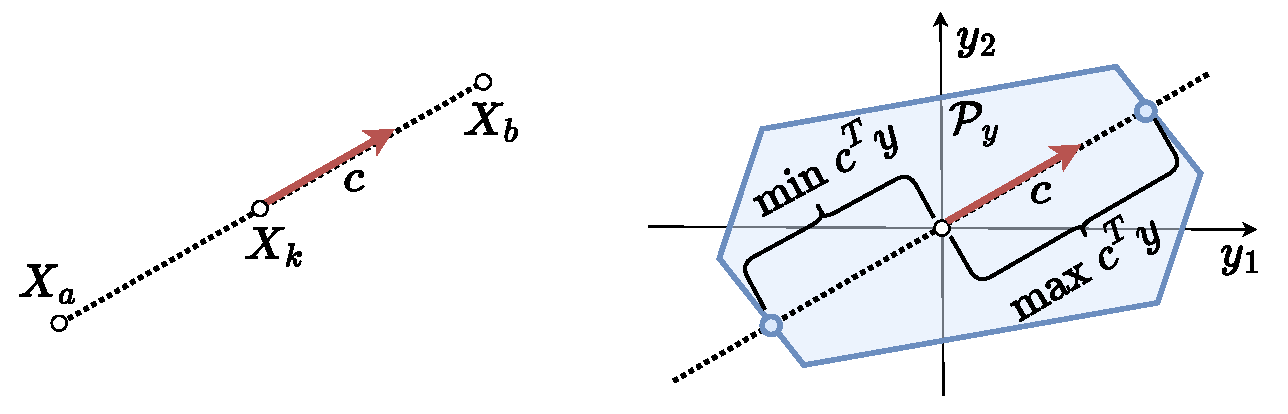
\includegraphics[width=0.7\linewidth]{Papers/imgs/dirs.pdf}
    \caption{Figure demonstrating the proposed approach to finding the maximal \gls{cs} capacity in the path direction. Robot's path is shown on the left and where the path direction vector $\bm{c}$ is shown in red. Polytope $\mathcal{P}_y$ of the \gls{cs} capacity is shown in blue on the right. The maximal and minimal capacity in the path direction can then be found by minimising and maximising the \gls{lp} defined in (\ref{eq:lp_general}).}
    \label{fig:normal_lp}
\end{figure}
With the known path direction $\bm{c}$ and the path normal space projector $N$, the maximal value of the Cartesian variable $\bm{y} \in\mathbb{R}^m$, in the path direction $\bm{c}$, within its range expressed as a convex polytope $\mathcal{P}_y$, can be found by solving the \gls{lp} \cite{vajda_gass_1964}
% \begin{equation}
% \begin{split}
%     \max_{\bm{y}} ~c^T \bm{y}&\\
%     s.t. ~ V_2^T\bm{y} &= \bm{0}\\
%     \bm{y}&\in \mathcal{P}_y
% \end{split}\label{eq:lp_general}
% \end{equation}
\begin{equation}
\begin{split}
    \max_{\bm{y}} ~\bm{c}^T \bm{y}& \\
    s.t. ~ N\bm{y} &= \bm{0}, \\
    \bm{y}&\in \mathcal{P}_y
\end{split}\label{eq:lp_general}
\end{equation}
whereas the minimum can be found by minimising it. \Cref{fig:normal_lp} illustrates geometrically this procedure.

By substituting the generic Cartesian variable $\bm{y}$ with Cartesian velocity $\dot{\bm{x}}$, acceleration $\ddot{\bm{x}}$ and jerk $\dddot{\bm{x}}$ and its polytope $\mathcal{P}_y$  with their respective polytopic limits (\ref{eq:limits_poly}), \gls{lp} formulation (\ref{eq:lp_general}) can be directly used to calculate the limits of the velocity $\dot{s}$, acceleration $\ddot{s}$ and jerk $\dddot{s}$ in the trajectory direction $\bm{c}$.  

\paragraph*{Cartesian velocity example} When searching for maximal Cartesian velocity $\dot{s}_{max}$, assuming known robot configuration $\bm{q}_k$ and trajectory direction vector $\bm{c}$, the Cartesian velocity along the trajectory $\dot{s}$ can be calculated as a projection of the Cartesian velocity $\dot{\bm{x}}$ 
\begin{equation}
    \dot{s} = \bm{c}^T\dot{\bm{x}}= \bm{c}^TJ(\bm{q}_k)\dot{\bm{q}} = \bm{c}^TJ(\bm{q}_k)\dot{\bm{q}} + \bm{c}^T\bm{b}_v
\end{equation}
where $\bm{b}_v \in \mathbb{R}^m$ is a zero vector. Substituting this relationship into the \gls{lp} formulation (\ref{eq:lp_general}) yields 
\begin{equation}
\begin{split}
    \dot{s}_{max} = \max_{\dot{\bm{q}}} \bm{c}^TJ(\bm{q}_k)\dot{\bm{q}} &+ \bm{c}^T\bm{b}_v  \\
    s.t.\quad NJ(\bm{q}_k)\dot{\bm{q}} &= - N\bm{b}_v, \\
    \dot{\bm{q}}&\in [\dot{\bm{q}}_{min}, \dot{\bm{q}}_{max}]
\end{split}\label{eq:lp_vel_max}
\end{equation}

The equivalent \gls{lp} expressions for finding the maximal acceleration and jerk are obtained by substituting $\dot{\bm{q}}$ and $\bm{b}_v$ with $\ddot{\bm{q}}$, $\bm{b}_a$ and $\dddot{\bm{q}}$, $\bm{b}_j$. The minimal values are found by minimising the same problem.
Therefore, using the proposed procedure, for any path direction $\bm{c}$ and a given robot state $\{\bm{q}_k, \dot{\bm{q}}_k, \ddot{\bm{q}}_k\}$, the robot's movement capacities (velocity $\dot{s}$, acceleration $\ddot{s}$ and jerk $\dddot{s}$) in the path direction can be expressed as
\begin{equation}
\begin{split}
    \dot{\bm{s}} &\in [\dot{\bm{s}}_{min}(\bm{q}_k),~ \dot{\bm{s}}_{max}(\bm{q}_k) ]\\
    \ddot{\bm{s}} &\in [\ddot{\bm{s}}_{min}(\bm{q}_k, \dot{\bm{q}}_k),~ \ddot{\bm{s}}_{max}(\bm{q}_k, \dot{\bm{q}}_k) ]\\
    \dddot{\bm{s}} &\in [\dddot{\bm{s}}_{min}(\bm{q}_k, \dot{\bm{q}}_k, \ddot{\bm{q}}_k),~ \dddot{\bm{s}}_{max}(\bm{q}_k, \dot{\bm{q}}_k, \ddot{\bm{q}}_k) ]
\end{split}
\label{eq:range_in_path_direction}
\end{equation}
Therefore, determining the robot's instantaneous movement capacity in the path direction can be obtained very efficiently, by solving a sequence of 6 \gls{lp} problems and allowing for real-time execution.

\subsection{Integrating task induced Cartesian space limits}

In many cases, when planning for \gls{cs} movement, the task requires limiting maximal \gls{cs} velocity, acceleration and jerk. For example, when executing trajectories in the human vicinity, it is common practice to limit the robot's \gls{cs} velocity $\dot{\bm{x}}$ to minimise the potential impact forces due to the robot's moment of inertia \cite{smu} and kinetic energy \cite{joseph2020}.
On the other hand, when designing trajectories of robotic manipulation of liquids, in order to prevent its sloshing or spilling, translation acceleration $\ddot{\bm{x}}$ continuity needs to be ensured \cite{moriello2018}, which in term corresponds to introducing \gls{cs} jerk $\dddot{\bm{x}}$ limits.

Therefore, if an additional task specific limit of a \gls{cs} variable $\bm{y}$ (velocity, acceleration or jerk) is required that can be expressed as an interval
\begin{equation}
\bm{y}\in  [\bm{y}_{min},~\bm{y}_{max}]\label{eq:limits_cs_additional}
\end{equation}
or more generally in a form of polytope defined by a set of inequality constraints
\begin{equation}
\mathcal{C} = \left\{ \bm{y} ~|~ A \bm{y} \leq \bm{b} \right\}
\label{eq:Cartesian_polytope_additional}
\end{equation}
Then the \gls{lp} problem (\ref{eq:lp_general}) can be extended to account for the polytope (\ref{eq:Cartesian_polytope_additional})
\begin{equation}
\begin{split}
    \max_{\bm{y}} ~c^T \bm{y}& \\
    s.t. ~ N\bm{y} &= \bm{0}, \\
    \bm{y}&\in \mathcal{P}_y \cap \mathcal{C}
\end{split}\label{eq:lp_general_additional}
\end{equation}
% \todo[inline]{I could maybe add inequality constraints rather than put this intersection $\mathcal{P}_y \cap \mathcal{C}$}

\paragraph*{Cartesian velocity example} Following the same example of maximal velocity $\dot{s}_{max}$ along the trajectory from (\ref{eq:lp_vel_max}), if an additional \gls{cs} limits are imposed by the task 
\begin{equation}
\mathcal{C}_v = \left\{ \dot{\bm{x}} ~|~ A \dot{\bm{x}} \leq \bm{b} \right\}
\label{eq:example_vel_poly}
\end{equation}
the maximal velocity $\dot{s}_{max}$ along the trajectory that respects both task constraint (\ref{eq:example_vel_poly}) and robot's instantaneous movement capacity (\ref{eq:vel_poly}), can be found by extending the \gls{lp} formulation (\ref{eq:lp_vel_max})
\begin{equation}
\begin{split}
    \dot{s}_{max} = \max_{\dot{\bm{q}}} \bm{c}^TJ(\bm{q}_k)\dot{\bm{q}} &+ \bm{c}^T\bm{b}_v  \\
    s.t.\quad NJ(\bm{q}_k)\dot{\bm{q}} &= - N\bm{b}_v, \\
    AJ(\bm{q}_k)\dot{\bm{q}} &\leq \bm{b} - A\bm{b}_v, \\
    \dot{\bm{q}}&\in [\dot{\bm{q}}_{min}, \dot{\bm{q}}_{max}]
\end{split}\label{eq:lp_vel_max_additional}
\end{equation}

The lower limit $\dot{s}_{min}$ can be found by minimising the same problem. T

% \todo[inline]{Should I talk about acceleration and jerk?}

\subsection{Scaling robot's Cartesian space limits}
% \todo[inline]{optional}

When it comes to planning robot trajectories, it is a common practice to consider only a part (certain percentage) of the specified robot limits. This is partially due to the fact that more dynamic robot movements require higher actuation capacity and leave less margin to account for potential tracking error, in many cases resulting in impaired tracking performance and potentially even raise different safety concerns.

When the robot's \gls{cs} kinematic limits are assumed constant, the simplest form of scaling can be done by multiplying the specified limits with scalar factors $\alpha_v,\alpha_a,\alpha_j\in[0,1]$.
\begin{equation}
\begin{split}
\dot{\bm{x}}&\in  [\alpha_v\dot{\bm{x}}_{min},~\alpha_v\dot{\bm{x}}_{max}] \\
\ddot{\bm{x}}&\in  [\alpha_a\ddot{\bm{x}}_{min},~\alpha_a\ddot{\bm{x}}_{max}] \\
\dddot{\bm{x}}&\in  [\alpha_j\dddot{\bm{x}}_{min},~\alpha_j\dddot{\bm{x}}_{max}] \\
 \end{split} \label{eq:limits_cs_alpha}
\end{equation}
allowing the robots velocity $\dot{\bm{x}}$, acceleration $\ddot{\bm{x}}$ and jerk $\dddot{\bm{x}}$ not to exceed certain percentage of the specified limits. 

However, if the robot's \gls{cs} kinematic capacity is not considered constant, but a result of the robot's current state $\{\bm{q},\ddot{\bm{q}},\ddot{\bm{q}}\}$, and its \gls{js} kinematic limits (\ref{eq:topca_kin_limits}), then the scaling using the scalars $\alpha_v,\alpha_a,\alpha_j\in[0,1]$ can done in the \gls{js}
\begin{equation}
\begin{split}
\dot{\bm{q}}&\in  [\alpha_v\dot{\bm{q}}_{min},~\alpha_v\dot{\bm{q}}_{max}] \\
\ddot{\bm{q}}&\in  [\alpha_a\ddot{\bm{q}}_{min},~\alpha_a\ddot{\bm{q}}_{max}] \\
\dddot{\bm{q}}&\in  [\alpha_j\dddot{\bm{q}}_{min},`\alpha_j\dddot{\bm{q}}_{max}] \\
 \end{split} \label{eq:limits_js_alpha}
\end{equation}
These new modulated \gls{js} limits can then be used to calculate the polytopes $\mathcal{P}_v$,$\mathcal{P}_a$ and $\mathcal{P}_j$ using equations (\ref{eq:vel_poly}-\ref{eq:jerk_acc_poly}), and in term scale the robot's \gls{cs} movement capacity in path direction (\ref{eq:range_in_path_direction}). 

\section{Cartesian space trajectory planning accounting for evolving capacity}
\label{ch:tap}


In order to fully exploit the robot's changing movement capacity while executing the trajectory, this work proposes a real-time re-planning strategy.
The proposed trajectory planning method leverages the computational efficiency of \gls{tap} or S-curve velocity profiles \cite[Chapter 9.2.2.2]{modernrobotics}\cite{scurve,ruckig}, a classical approach to finding the \gls{cs} time-optimal or minimum-time trajectories \cite{Gasparetto2012}. 
In each step of the trajectory execution, the proposed method evaluates the robot's movement capacity in the path direction, using the efficient method described in \Cref{ch:capacity_lp}, and recalculates the new time-optimal trajectory using \gls{tap} planning on the remaining path. 

The following section, \Cref{ch:tap}, brings a brief introduction to the basics of the \gls{tap} planning, while \Cref{ch:update_cap} provides more details about the real-time re-planning approach. 
 
\subsection{Trapezoidal acceleration profile basics}

\gls{cs} point-to-point straight-line paths connect two \gls{cs} poses $X_a$ and $X_b$ (for example expressed as homogeneous matrices in $SE(3)$) of the desired robot's frame (ex. end-effector frame) \cite[Chapter 9.2.1]{modernrobotics}. These paths can be expressed as $\mathscr{P}(s)$, where $s\in\left[0,d\right]$ is a scalar position on the path with a length $d$ \cite{Constantinescu2000,Pfeiffer1987}. 

\begin{wrapfigure}{r}{0.4\linewidth}
\vspace{-0.5cm}
    \centering
    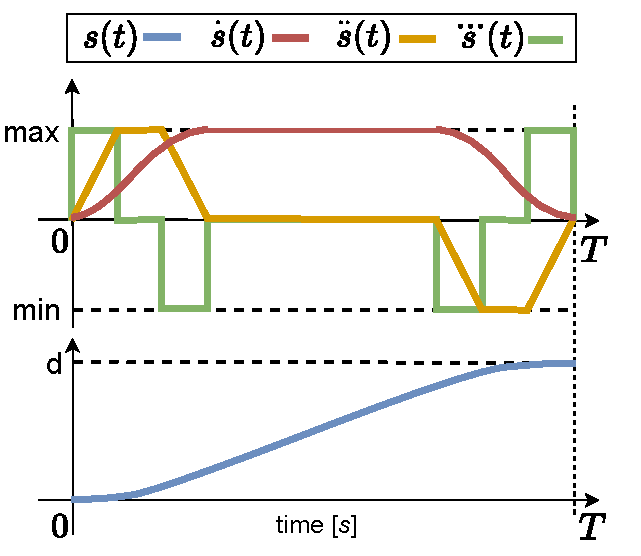
\includegraphics[width=\linewidth]{Papers/imgs/tap_profile.pdf}
    \caption{\gls{tap} example, all the initial and final conditions are set to 0.}
    \label{fig:tap_profile}
\end{wrapfigure}
When is comes to finding the time-optimal time evolution of the robot's \gls{cs} pose $X(t)$ following the straight line path between $X_a$ and $X_b$, one of the most common approaches in the literature are the \gls{tap} planning techniques \cite[Chapter 9.2.2.2]{modernrobotics}. \gls{tap} trajectory planning finds the time-optimal evolution of the path position variable $s(t)$ respecting the limits on all its derivatives
\begin{equation}
\begin{split}
    \dot{s} \in [\dot{s}_{min}, &\dot{s}_{max}], \quad
\ddot{s}\in [\ddot{s}_{min}, \ddot{s}_{max}], \\
\dddot{s}&\in [\dddot{s}_{min}, \dddot{s}_{max}] 
\end{split}\label{eq:s_limits}
\end{equation}
as well as the starting and end conditions 
\begin{equation}
    \dot{s}(0) = \dot{s}_{0} \quad \dot{s}(T) = \dot{s}_{T} \quad
    \ddot{s}(0) = \ddot{s}_{0} \quad \ddot{s}(T) = \ddot{s}_{T}
\end{equation}
Where $T$ is the trajectory duration, $\dot{s}_{0}$ and $\ddot{s}_{0}$ represent the velocity and acceleration at the beginning of the path $\mathscr{P}(s)$, while the $\dot{s}_{T}$ and $\ddot{s}_{T}$ represent their final values at the end of the trajectory. One example of the \gls{tap} profile is shown on \Cref{fig:tap_profile}.


When planing for the geometric paths $\mathscr{P}(s)$ in \gls{cs}, where the \gls{cs} poses $X_a$ and $X_b$ belong to $SE(3)$, it is common practice to separate the translation $\mathscr{P}_t(s_t)$ and orientation $\mathscr{P}_r(s_r)$ component of the path $\mathscr{P}(s)$\cite{Bobrow1985}. The translation component of the path can then be expressed as
\begin{equation}
    \mathscr{P}_t(s_t) = s_t \bm{u}_t, \quad s_t \in \left[0, ||X_{b}^t - X_{a}^t||_2\right]\label{eq:trans_path}
\end{equation}
where $X_{a}^t$ and $X_{b}^t$ are the translation parts of the poses $X_a$ and $X_b$ and $\bm{u}_t$ is the unit vector pointing from $X_{a}^t$ to $X_{b}^t$. For the orientation, the common approach is to use the axis-angle representation of the rotation, and specify the difference in orientation between $X_a$ and $X_b$ as an angle $\theta$ around the axis $\bm{u}_{r}$. Then the geometric path corresponding to the orientation $\mathscr{P}_o(s_r)$ can be written as
\begin{equation}
    \mathscr{P}_r(s_r) = s_r \bm{u}_{r}, \quad s_r \in \left[0, \theta\right] \label{eq:rot_path}
\end{equation}
$\mathscr{P}_r(s_r)$ and $\mathscr{P}_t(s_t)$ represent a relative change in the orientation and translation over the course of the trajectory from the initial pose $X_a$. The desired \gls{cs} pose $X(t)$ can be calculated using an homogeneous transformation matrix $H$, constructed from $\mathscr{P}_r$ and $\mathscr{P}_t$ 
\begin{equation}
    X(t) = X_a H\Big(\mathscr{P}_r\big(s_r(t)\big), ~\mathscr{P}_t\big(s_t(t)\big)\Big)
\end{equation}
and optimal \gls{cs} velocity and acceleration can be found
\begin{equation}
    \dot{\bm{x}}(t)= \begin{bmatrix}\dot{s}_t(t) \bm{u}_t \\ \dot{s}_r( t) \bm{u}_r\end{bmatrix}, \quad 
    \ddot{\bm{x}}(t)= \begin{bmatrix}\ddot{s}_t(t) \bm{u}_t \\ \ddot{s}_r(t) \bm{u}_r\end{bmatrix}
\end{equation}

% Cartesian $\dot{\bm{x}}$, acceleration $\ddot{\bm{x}}$ and jerk $\dddot{\bm{x}}$ limits (\ref{eq:limits_cs}) can then be projected on the path transforming them to limits on the trajectory variables $s_r(t)$ and $s_t(t)$, using vectors $\bm{c}_t = [\bm{u}_t^T, \bm{0}_{3\times 1}]^T$ and $\bm{c}_r =[\bm{0}_{3\times 1}, \bm{u}_r^T]^T$
% \begin{equation}
% \begin{split}
% \bm{c}^T_i\dddot{\bm{x}}_{min} \leq \dddot{\bm{s}}_i(t)&  \leq  \bm{c}^T_i\dddot{\bm{x}}_{max} \\
% \bm{c}^T_i\ddot{\bm{x}}_{min} \leq \ddot{\bm{s}}_i(t)&  \leq \bm{c}^T_i\ddot{\bm{x}}_{max} \\
% \bm{c}^T_i\dot{\bm{x}}_{min} \leq \dot{\bm{s}}_i(t)&  \leq \bm{c}^T_i\dot{\bm{x}}_{max}\\
%  \end{split} \label{eq:limits_s_cs}
% \end{equation}
% where $i$ is either the translation $t$ or the orientation $o$.

%\DD{Etre plus précsis dans les equations qui melangent translation et orientation, $c_i$ semble être de dimension 3}

The translation path $\mathscr{P}_t(s_t)$ and the orientation path $\mathscr{P}_r(s_r)$ direction can be calculated as 
\begin{equation}
    \bm{c}_t = [\bm{u}_t^T, \bm{0}_{3\times 1}]^T, \qquad \bm{c}_r =[\bm{0}_{3\times 1}, \bm{u}_r^T]^T
    \label{eq:directions_path}
\end{equation}
where $\bm{u}_t\in\mathbb{R}^3$ is the unit vector pointing from the \gls{cs} pose $X_a^t$ to $X_b^t$ and $\bm{u}_r\in\mathbb{R}^3$ represents the axis of the rotation between the poses.

Once both translation and orientation \gls{tap} trajectories are found resulting in optimal $s_r(t)$ and $s_t(t)$, to synchronise the two movements, their time duration is matched, making both trajectories last the same time $T$, the time taken by the longer of the two trajectories $T = \max\{T_r,T_t\}$. 

The inherent challenge of \gls{tap} planning for the robot's motion in the \gls{cs} is that its movement capacity limits (\ref{eq:s_limits}) are robot's state dependent, and over the course of the trajectory the robot's movement capacity can change significantly. Therefore, no set of fixed \gls{cs} limits as defined in (\ref{eq:s_limits}) will be able to exploit the robot's full movement capabilities.  

% \todos{Lie algebra solution without separation - not straight line motion. Put in a remark.}

\subsection{Allowing for real-time updates of CS capacity}
\label{ch:update_cap}



% As discussed in \Cref{ch:capacity} robot's \gls{cs} movement capacity evolves in real-time with the changes in it's state $\{\bm{q}, \dot{\bm{q}}, \ddot{\bm{q}}\}$ and can be represented in a polytope form
% \begin{equation}
%     \dot{\bm{x}}\in \mathcal{P}_v(\bm{q}), \quad \ddot{\bm{x}}\in \mathcal{P}_a(\bm{q},\dot{\bm{q}}), \quad \dddot{\bm{x}}\in \mathcal{P}_j(\bm{q},\dot{\bm{q}},\ddot{\bm{q}})\label{eq:limits_poly}
% \end{equation}
% With the assumption of the point-to-point straight line \gls{cs} paths, the polytope shaped limits can be simplified, by projecting them in the path direction. The efficient approach of determining the robot's movement capacity in the path direction is described in \Cref{ch:capacity_lp}, resulting in min-max ranges of corresponding to the robot's limits of achievable scalar velocity $\dot{s}\in\mathbb{R}$, acceleration $\dot{s}\in\mathbb{R}$ and jerk $\dot{s}\in\mathbb{R}$ in the path direction
% \begin{equation}
% \begin{split}
%     \dot{\bm{s}} &\in [\dot{\bm{s}}_{min}(\bm{q}),~ \dot{\bm{s}}_{max}(\bm{q}) ]\\
%     \ddot{\bm{s}} &\in [\ddot{\bm{s}}_{min}(\bm{q}, \dot{\bm{q}}),~ \ddot{\bm{s}}_{max}(\bm{q}, \dot{\bm{q}}) ]\\
%     \dddot{\bm{s}} &\in [\dddot{\bm{s}}_{min}(\bm{q}, \dot{\bm{q}}, \ddot{\bm{q}}),~ \dddot{\bm{s}}_{max}(\bm{q}, \dot{\bm{q}}, \ddot{\bm{q}}) ]
% \end{split}
% \label{eq:range_in_path_direction_revisit}
% \end{equation}

\begin{figure}[t]
    \centering
    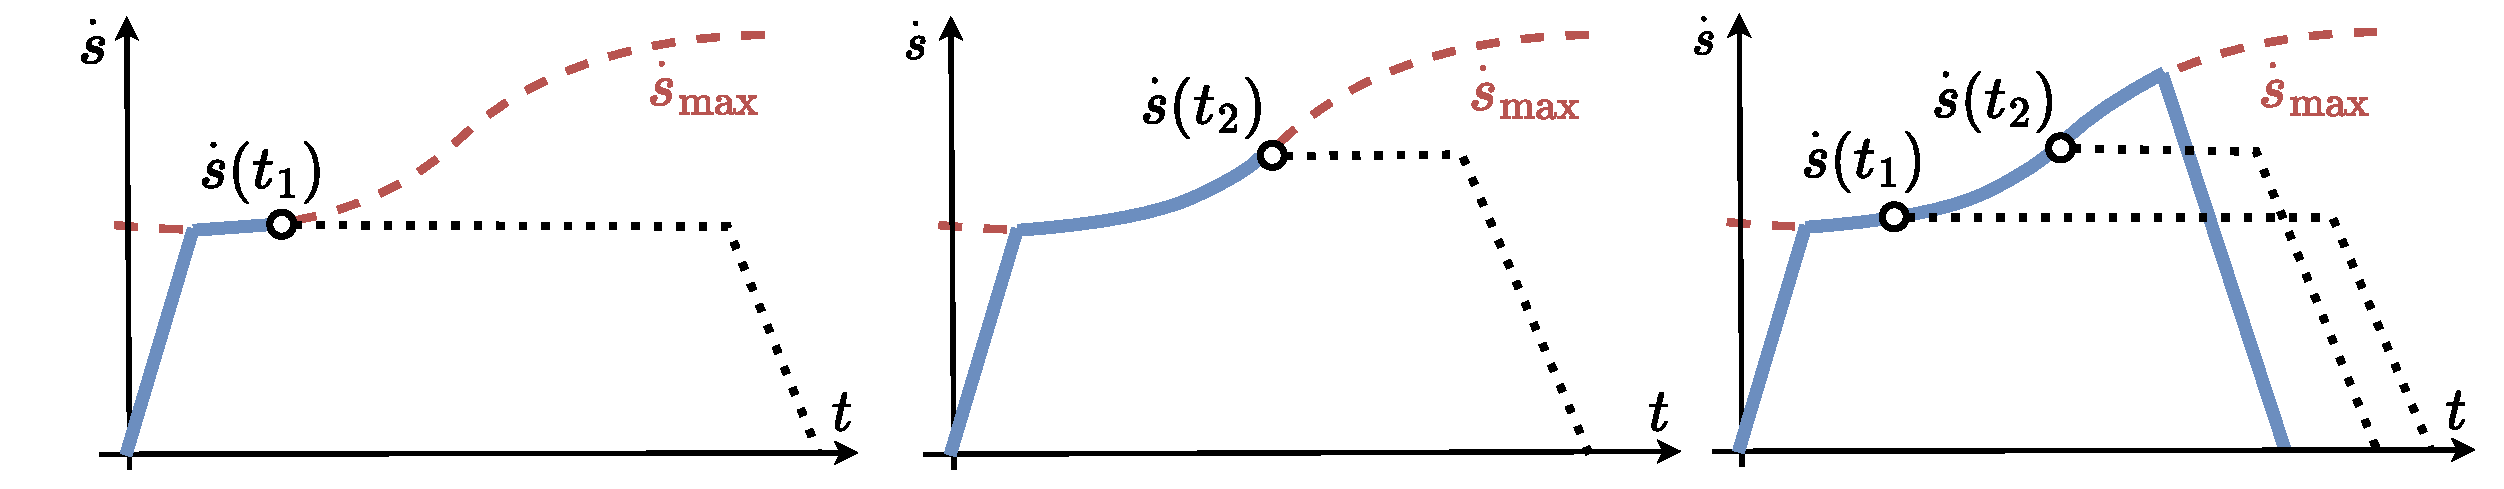
\includegraphics[width=\linewidth]{Papers/imgs/tap_replanning3.pdf}
    % 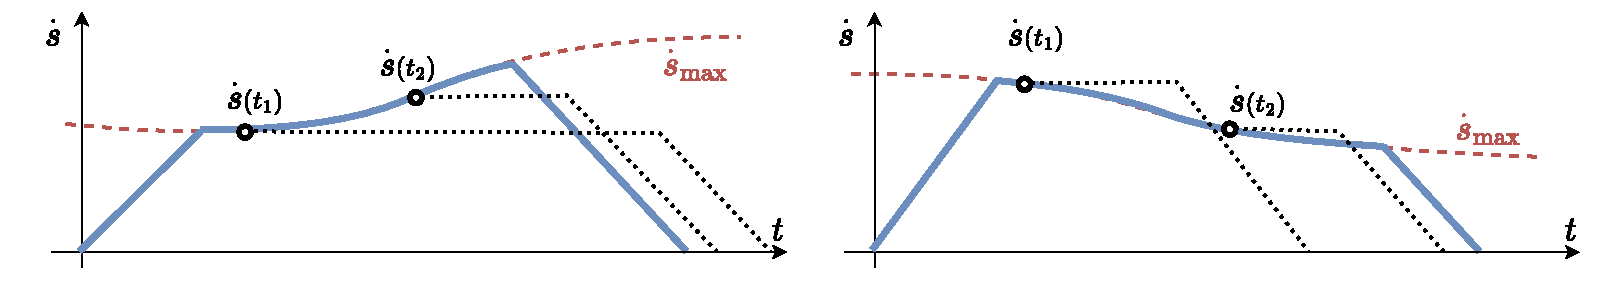
\includegraphics[width=\linewidth]{Papers/imgs/ICRA2023.drawio (25).pdf}
    \caption{Velocity curve, updated in the real time with instantaneous maximal values. At each time-step $t_k$ during the trajectory execution (ex. $t_1$ and $t_2$) the \gls{tap} planning calculates the remaining trajectory considering that maximal velocity $\dot{s}_{max}$ constant till the end of the movement (black dotted lines). As the maximal velocity $\dot{s}_{max}$ increases during the trajectory execution (red dashed line), the final trajectory duration is considerably shorter. }
    \label{fig:replanning}
\end{figure}

To address the issue of constantly changing kinematic limits (\ref{eq:s_limits}), during robot trajectory execution, a real-time re-planning strategy is proposed. This approach consists in evaluating the jerk $\dddot{s}$, acceleration $\ddot{s}$ and velocity $\dot{s}$ limits at each step of the trajectory execution, using the proposed method in \Cref{ch:capacity_lp}. 
The updated limits are then considered constant until the end of the movement and used in conjunction with the \gls{tap} algorithm to calculate the time-optimal profile of the remaining trajectory.  
\Cref{fig:replanning} illustrates the proposed approach on the example of the velocity $\dot{s}$ curve. 


In each time step $k$, corresponding to the moment in time $t_k$ and robot's state $\{\bm{q}_k,\dot{\bm{q}}_k,\ddot{\bm{q}}_k\}$, the instantaneous limits on the path variables $s_r(t)$ and $s_t(t)$ are calculated using the method described in \Cref{ch:capacity_lp}. The new updated limits have a form
\begin{equation}
\begin{split}
    \dot{\bm{s}}_i &\in [\dot{\bm{s}}_{i,min}(\bm{q}_k),~ \dot{\bm{s}}_{i,max}(\bm{q}_k) ]\\
    \ddot{\bm{s}}_i &\in [\ddot{\bm{s}}_{i,min}(\bm{q}_k, \dot{\bm{q}}_k),~ \ddot{\bm{s}}_{i,max}(\bm{q}_k, \dot{\bm{q}}_k) ]\\
    \dddot{\bm{s}}_i &\in [\dddot{\bm{s}}_{i,min}(\bm{q}_k, \dot{\bm{q}}_k, \ddot{\bm{q}}_k),~ \dddot{\bm{s}}_{i,max}(\bm{q}_k, \dot{\bm{q}}_k, \ddot{\bm{q}}_k) ]
\end{split}
\label{eq:range_in_path_direction_revisit}
\end{equation}
where $i$ is either the translation $t$ or the orientation $r$. The translation limits are calculated using the direction vector $\bm{c}_t$ and the rotation limits are calculated using $\bm{c}_r$, defined in (\ref{eq:directions_path}). 

Then, given the robot's position on the trajectory $s_t(t_k),s_r(t_k)$, the remaining length of the geometric path to the target position can be calculated as $d_k = s_{t,T} - s_t(t_k)$ and the remaining angle of rotation $\theta_k\!=\!s_{r,T}\! - \!s_r(t_k)$. Then the initial conditions for the new planning execution can be updated 
\begin{equation}
\begin{split}
    s_t \in [0, d_k], \quad \dot{s}_{t,0} = \dot{s}_t(t_k), \quad \ddot{s}_{t,0} = \ddot{s}_t(t_k),\\ 
    s_r \in [0 , \theta_k], \quad \dot{s}_{r,0} = \dot{s}_r(t_k), \quad \ddot{s}_{r,0} = \ddot{s}_r(t_k)
\end{split}\label{eq:rt_init}
\end{equation}

Finally, an updated \gls{tap} trajectory can then be calculated for the translation $s_t(t)$ and the orientation $s_r(t)$, resulting in an optimal robot trajectory given the updated robot's limits (\ref{eq:range_in_path_direction_revisit}) and the initial conditions (\ref{eq:rt_init}). 
The assumption of constant limits (\ref{eq:range_in_path_direction_revisit}) for the duration of the remaining trajectory is a simplification that might not hold true in practice, as the robot's movement capacity can change significantly over time. However, this issue is addressed through real-time planning, which constantly updates the plan using the latest information on the robot's current ability. The \gls{tap} planning algorithm is well-suited for this approach, as it is highly efficient in computing optimal trajectories, allowing for real-time execution. 

An example of the generated velocity $\dot{s}$ profile using real-time \gls{tap} re-planning, with constantly changing limits $\dot{s}_{max}$, is shown on \Cref{fig:replanning}. 

\section{Compensating for real-time TAP planning negative effects}
\label{ch:heuristics}
The proposed approach adapts to the constant changes of the robot's motion capabilities by planning the new \gls{tap} trajectory at each time step $t_k$. For each planning iteration it considers constant robot's capabilities until the end of the trajectory. This assumption is reasonable as only the first step of each planned trajectory is used, in which the calculated robot's capabilities are valid. 
However, based on the prediction of robot's constant movement capacity the \gls{tap} planning decides the phase of the trajectory, when to stop accelerating and when to start braking. Therefore, in some cases, especially when robot's capacity changes significantly towards the end of the trajectory, \gls{tap} planning can produce oscillations and an overshoot due to the switching between the modes of braking and accelerating.
 
There are two main scenarios that generate unwanted behaviour, both related to the robot's deceleration (braking) capacity. 
\Cref{ch:overshoot} describes the overshoot effect due to the robot's decreasing braking capacity towards the end of the trajectory, while \Cref{ch:oscillations} describes the oscillation effect produced by the robot's increasing braking capacity towards the end of the trajectory. The sections propose heuristics for minimising these effects and numerically validate the choice of their parameters.

\subsection{Decreasing braking capacity: Overshoot effect} 
\label{ch:overshoot}
\begin{wrapfigure}{r}{0.45\linewidth}
    \centering
    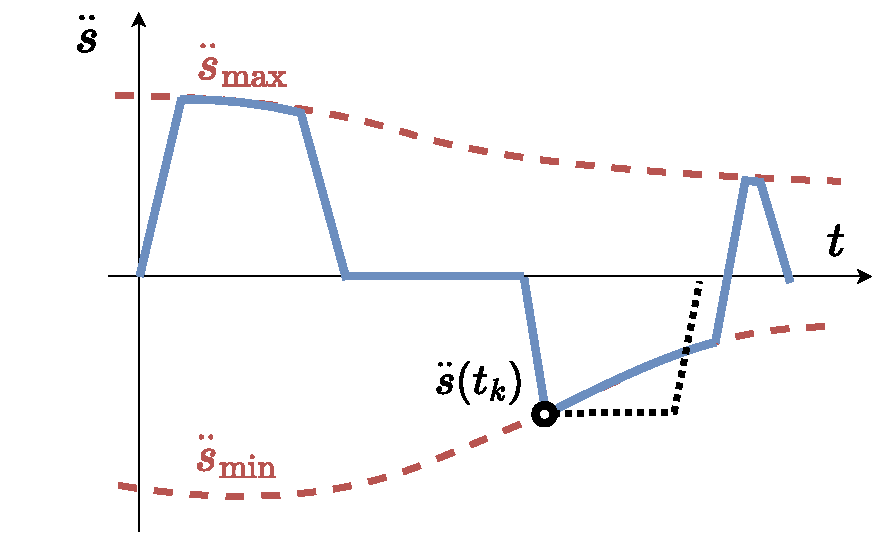
\includegraphics[width=\linewidth]{Papers/imgs/overshoot_expl.pdf}
    \caption{Figure shows the effect of diminishing braking capacity towards the end of the trajectory, where the end result is an overshoot. }
    \label{fig:overshoot_expl}
\end{wrapfigure}
When the robot's deceleration capacity decreases towards the end of the trajectory, \Cref{fig:overshoot_expl}, the planned trajectory will have an overshoot. Due to considering robot's capacity constant, robot's braking capacity is overestimated and when the \gls{tap} planning decides to start braking, at the time step $t_k$, it is already too late, the robot is not able to stop before it reaches the target position. 

This is an inherent challenge of real-time planning and cannot be solved without adding a degree of prediction of the robot's future capabilities. One such approach to mitigate the overshoot is to predict the robot's minimal braking capacity for the remaining \gls{cs} path $\mathscr{P}(s(t_i))$ until the end of the trajectory $ t_i \in \left[t_k, T\right]$ and use this value for \gls{tap} planning.
\begin{equation}
    \ddot{s}_{min} = \max \left\{\ddot{s}_{min}(t_i)\right\} \quad t_i \in \left[t_k ,~ T\right]
\label{eq:minimal_braking_capacity}
\end{equation}
This approach in many cases results in more conservative trajectories as the robot's braking capacity is underestimated, but at the same time it guarantees the overshoot removal. As the robot's braking capacity depends on its joint state $\{\bm{q},\dot{\bm{q}}\}$, finding the minimal braking capacity (\ref{eq:minimal_braking_capacity}) requires either knowing the exact robot's \gls{js} path until the end of the trajectory, which is by definition not known, or finding all the possible joint configurations the robot can be in on the remaining path, which is very long and not practical for most real-time applications.

In this work a sampling based approximation of (\ref{eq:minimal_braking_capacity}) is proposed based on sampling the remaining the \gls{cs} path (from the current pose $X_k$ to the final pose $X_b$) into $N$ posses $X_i\in SE(3)$. The most probable predictions \gls{js} configurations $\bm{q}_i$ at each of the poses $X_i$ is proposed to be found as the robot's inverse kinematics solution the closest to the current pose $\bm{q}_k$. Finally, the prediction of (\ref{eq:minimal_braking_capacity}) can be found as the minimal braking capacity among all the sampled ones $\ddot{s}_{i, min}$
\begin{equation}
    \ddot{s}_{min} = \max \left\{\ddot{s}_{0, min},~ \ldots,~ \ddot{s}_{N, min}\right \}
\end{equation}

%\todo[inline]{I am not talking about how to decide which joint velocity $\dot{\bm{q}}_i$ to use!}


\subsubsection*{Experimental validation of compensation parameters} 
\begin{figure}[!h]
    \centering
    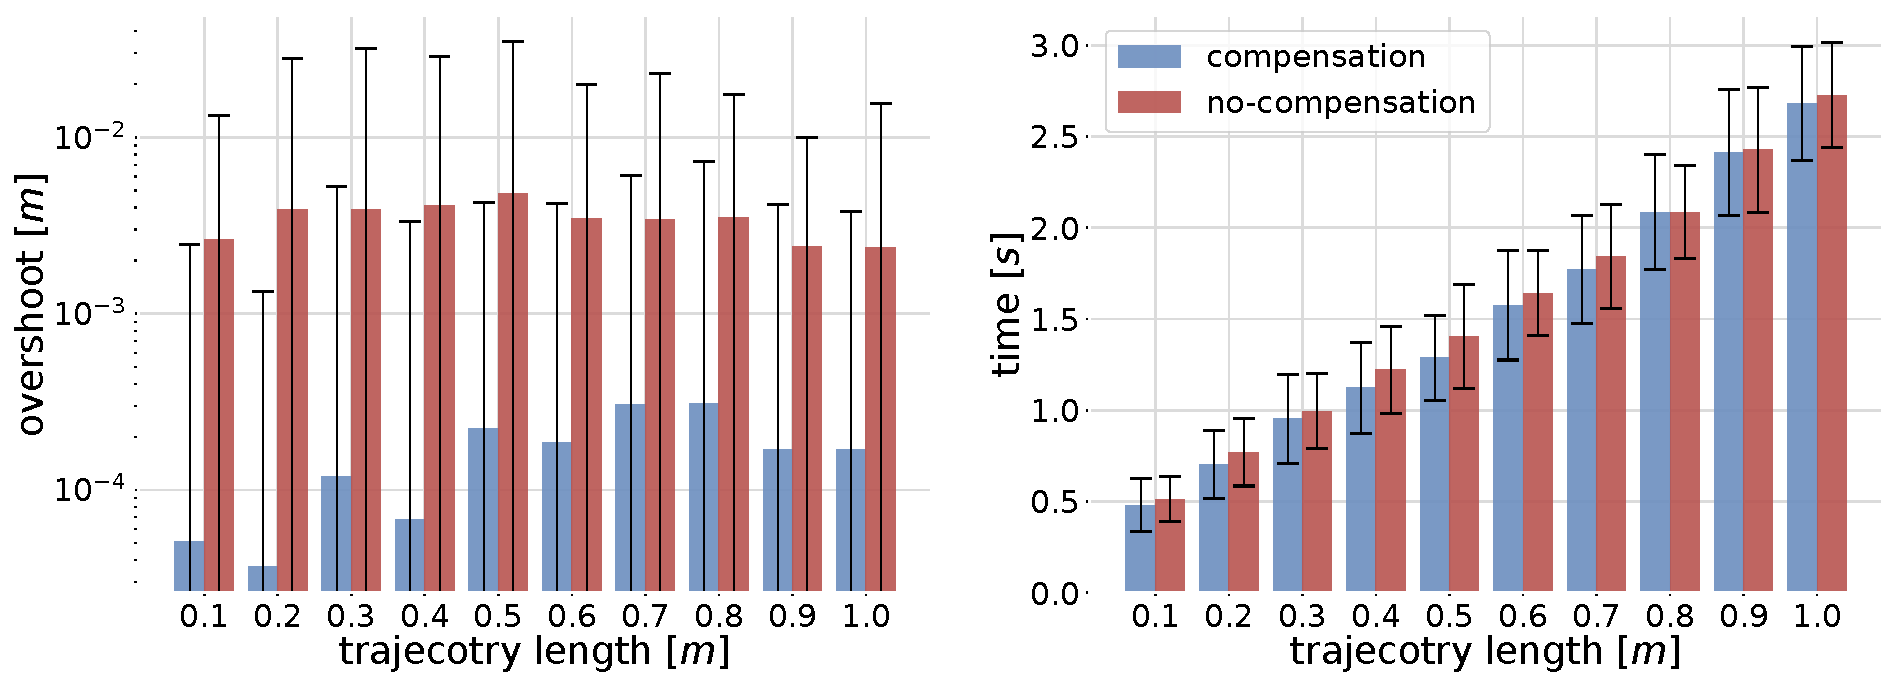
\includegraphics[width=\linewidth]{Papers/imgs/compensation_comp.pdf}
    \caption{Plots showing the comparison of the average overshoot (left) and average execution time (right) of the proposed method with and without overshoot compensation. For each length ranging from $d=0.1$ to $1m$, means and variances are calculated over 100 random trajectories. }
    \label{fig:compensatiopn_comp}
\end{figure}
In the experiments the remaining trajectory is sampled with $N=2$ points, corresponding to the current position $X_k$ in the time step $t_k$ and the final position at the end of the trajectory $X_T$. Joint configuration $\bm{q}_T$ at the $X_T$ is found as the inverse kinematics solution the closest to the current configuration $\bm{q}_k$ and the joint velocity $\dot{\bm{q}}_T$ and acceleration $\ddot{\bm{q}}_T$ are considered to be $\dot{\bm{q}}_T,\ddot{\bm{q}}_T= \bm{0}$, as the robot will come to a stop at the target $X_T$. Finally the braking capacity used for \gls{tap} planning in the step $t_k$ is the minimum of the two
\begin{equation}
    \ddot{s}_{min} = \max\left\{\ddot{s}_{k,min},~ \ddot{s}_{T,min}\right\}
\end{equation}

\Cref{fig:compensatiopn_comp} presents a comparison between the proposed method's performance with and without overshoot compensation. To evaluate the methods, 1000 random translation trajectories (random fixed orientation) were generated in the robot's workspace, ranging in length from $d\!=\!10cm$ to $d\!=\!1m$. The experiments were conducted in simulation using a Franka Emika Panda robot, the implementation details are described in \Cref{ch:setup}. The overshoot and execution time were recorded for each trajectory. The results indicate that the proposed method with overshoot compensation significantly reduces the expected overshoot compared to the method without compensation, going from $3mm$ average overshoot to $0.1mm$. Moreover, the compensation strategy does not have a negative impact on the trajectory execution time. On the contrary, it slightly reduces the average execution time, as shown in the figure.

The numerical analysis shows that even by taking in consideration only the final braking capacity of the robot $\ddot{s}_{T,min}$ the effects of the overshoot can be significantly reduced. Furthermore, as this strategy can be implemented very efficiently since the robot's final braking capacity $\ddot{s}_{T,min}$ has to be evaluated only once per trajectory execution. 

\subsection{Increasing braking capacity: Oscillations effect}
\label{ch:oscillations}
When the robot's breaking capacity increases along the trajectory, scenario shown on \Cref{fig:oscil_expl}, the proposed method can result in oscillatory behaviour.  Due to considering robot's capacity constant, robot's braking capacity is underestimated and the decision of the \gls{tap} planning to start braking, at the time step $t_k$, comes too soon. In the next step $t_{k+1}$ the robot's breaking capacity increases which makes \gls{tap}  planning take the decision to stop braking. The repetitions of this sequence create the oscillations of the planed acceleration profile and produces jerky trajectories. 

\begin{wrapfigure}{r}{0.45\linewidth}
    \centering
    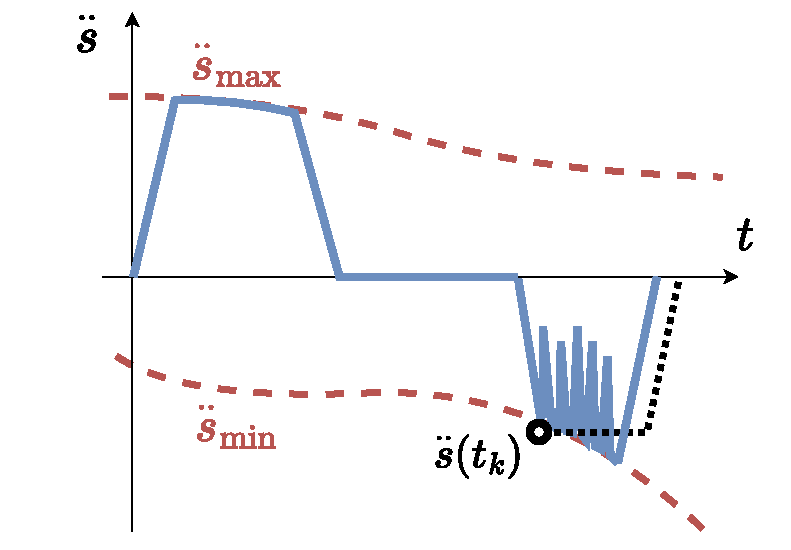
\includegraphics[width=\linewidth]{Papers/imgs/oscil_how_it_looks.pdf}
    \caption{Figure shows the effect of increasing braking capacity towards the end of the trajectory, where the end result are oscillations. }
    \label{fig:oscil_expl}
\end{wrapfigure}
The effect of these oscillations is greatly amplified as the robot's braking capacity $\ddot{s}_{min}$, is some cases, is inverse proportional to the robot's current joint velocity $\dot{\bm{q}}_{k}$ through the bias term $\bm{b}_a = \dot{J}(\bm{q}_k,\dot{\bm{q}}_k)\dot{\bm{q}}_k$. Lowering the the joint velocity $\dot{\bm{q}}_{k}$, lowers the bias $\bm{b}_a$ and increases the braking capacity $\ddot{s}_{min}$. This effect creates a closed loop behaviour, where more the robot brakes, more its braking capacity increases. \Cref{fig:overshoot_shema} illustrates few time steps of such oscillatory behaviour.

\begin{figure}[!t]
    \centering
    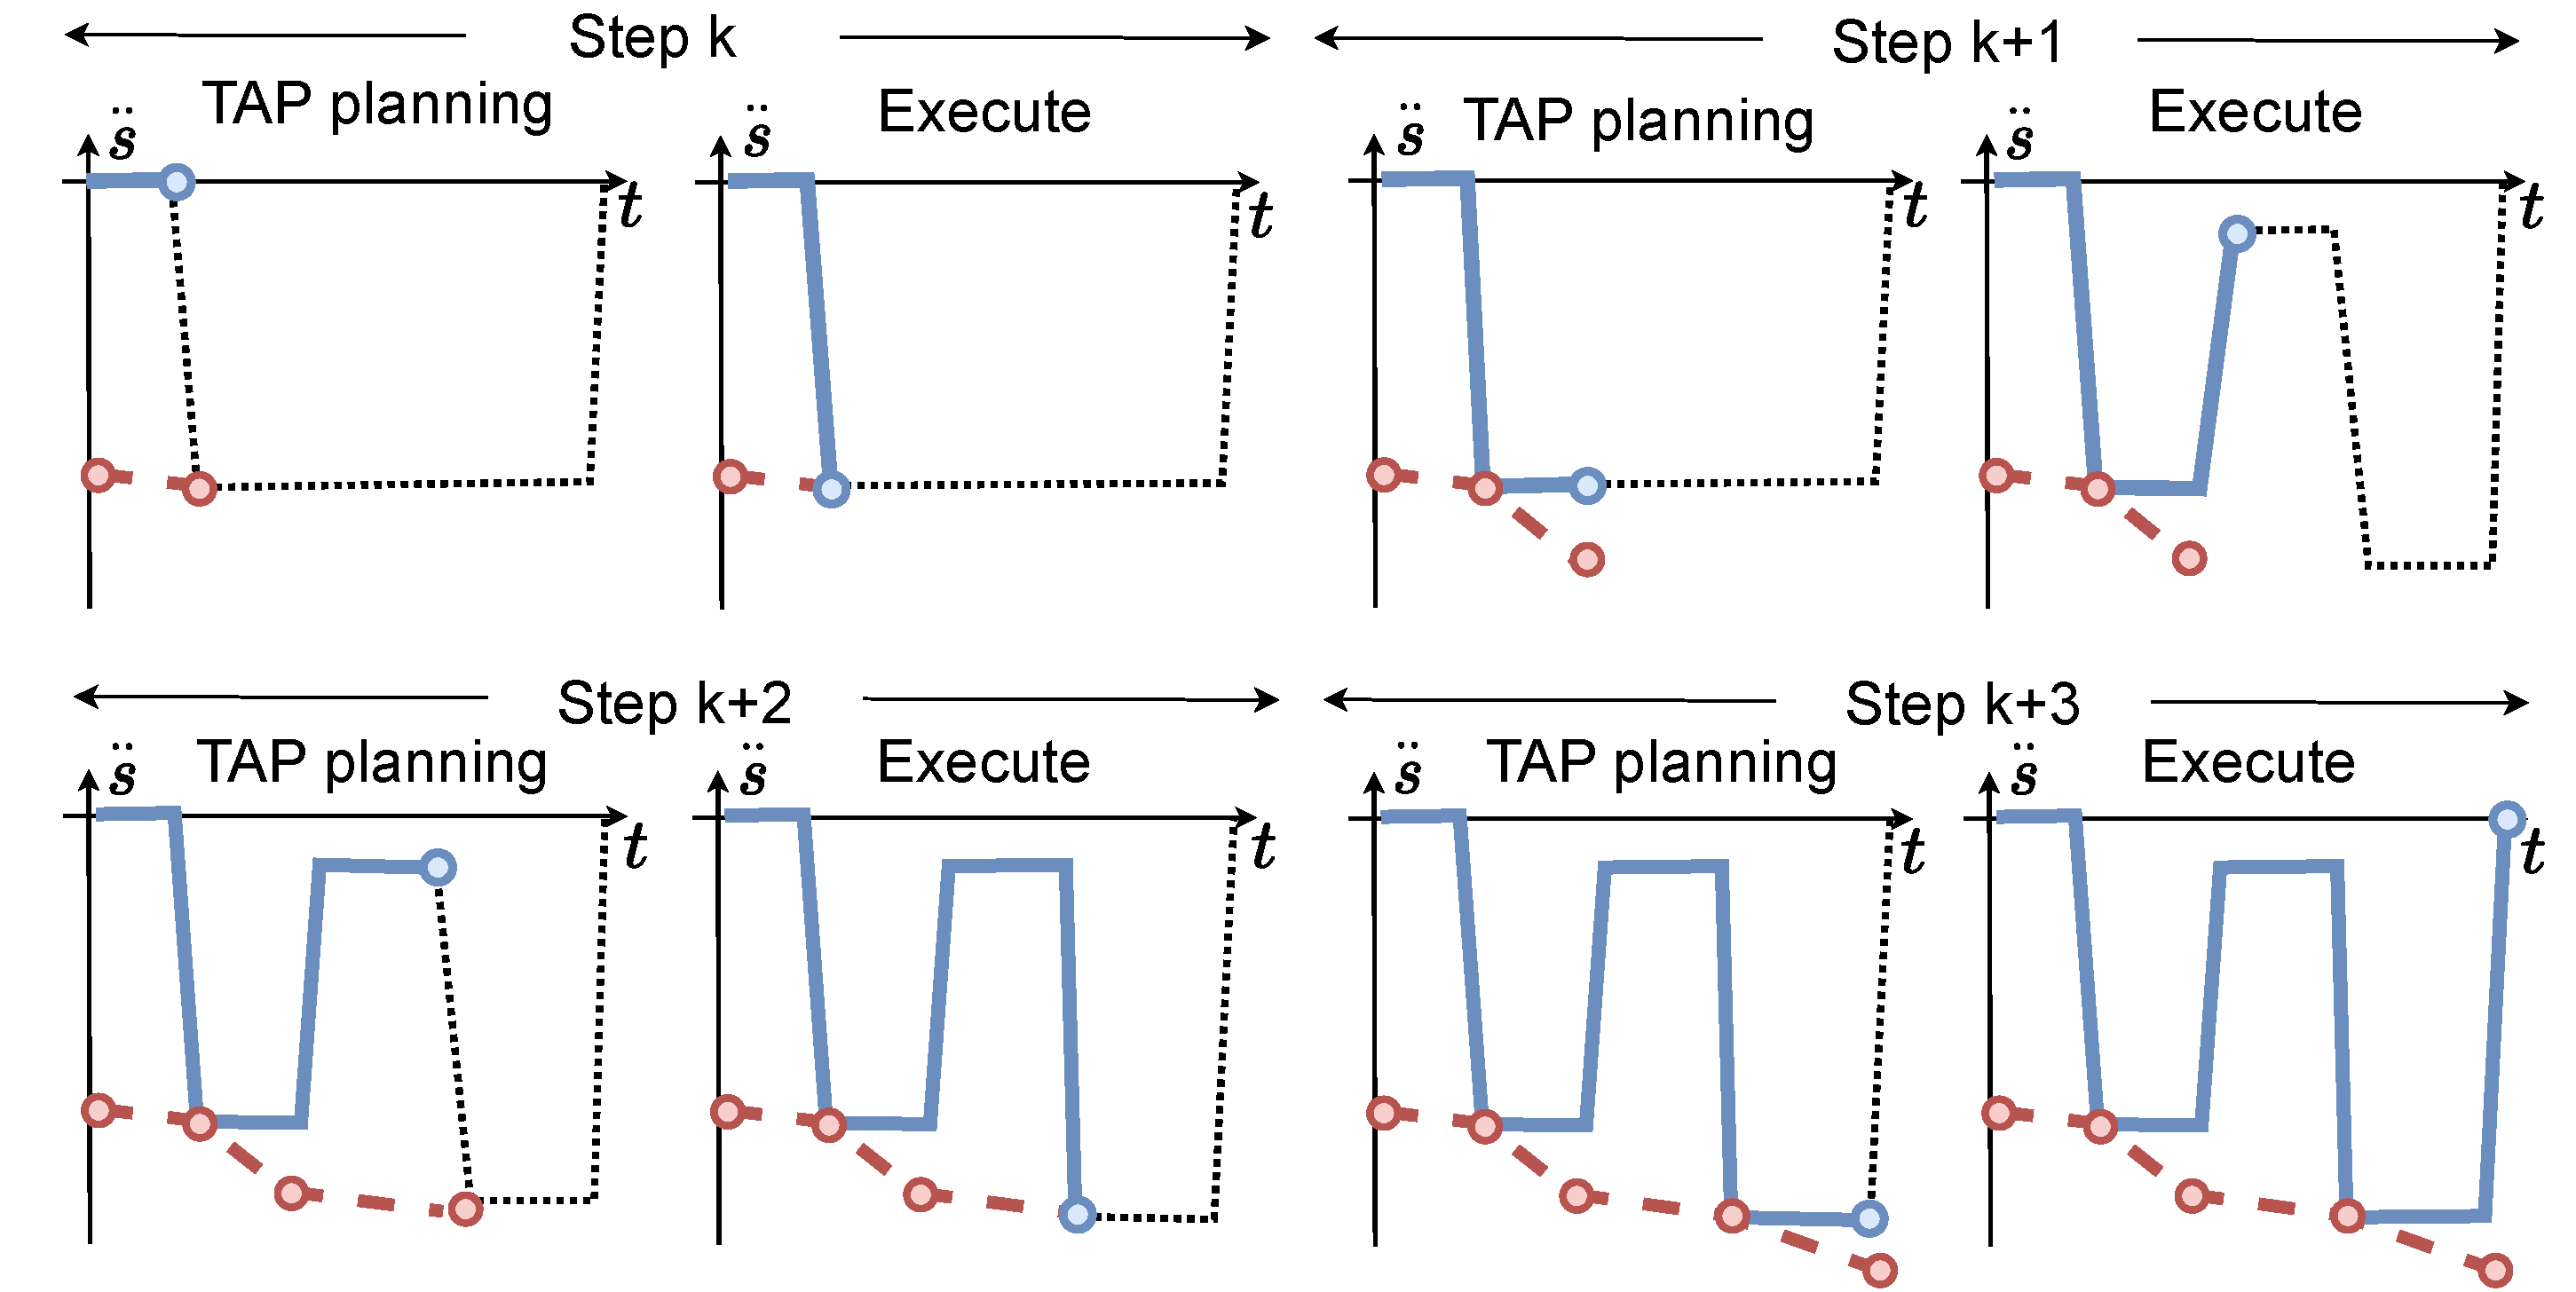
\includegraphics[width=\linewidth]{Papers/imgs/oscilation_expl.pdf}
    \caption{The figure shows braking stage of the \gls{tap} planning trajectory with the effect of augmenting braking capacity towards the end of the trajectory. The executed acceleration $\ddot{s}$ is shown in blue, the planned one is shown in black dotted lines and the maximal braking limit is shown in red dashed lines. Due to, in some cases, inverse proportional coupling between the robot's velocity $\dot{\bm{q}}$ and the braking capacity, more the robot brakes, more its velocity $\dot{\bm{q}}$ decreases and more the braking capacity increases. This effect produces an oscillatory behaviour, as shown in the sequence of figures. The robot starts braking in time step $k$. Because it was braking, its braking capacity increased in step $k+1$. With the increased braking capacity, \gls{tap} planning decides to decrease braking in step $n+1$ as it can brake stronger later.}
    \label{fig:overshoot_shema}
\end{figure}
In order to smooth the acceleration profile and reduce the effect of coupling introduced by the bias $\bm{b}_a$, a simple strategy is proposed which consists in down-sampling the \gls{tap} planning. Instead of planning the \gls{tap} trajectory in each time step $t_k$, the trajectory is planned with the time step $\Delta t_p$, while linearly interpolating the trajectory between the planning steps $t \in \left[t_k, t_k+\Delta t_p\right]$. 

\begin{equation}
    s(t) = s_k + \frac{s_{k+1}-s_k}{\Delta t_p}(t - t_k), \quad t \in \left[t_k, t_k + \Delta t_p\right]
\end{equation}
The same linear interpolation can be applied to the velocity $\dot{s}$ and acceleration $\ddot{s}$
\begin{equation}
\begin{split}
    \dot{s}(t) &= \dot{s}_k + \frac{\dot{s}_{k+1} - \dot{s}_{k}}{\Delta t_p}(t - t_k),\\
    \ddot{s}(t) &= \dot{s}_k + \frac{\ddot{s}_{k+1} - \ddot{s}_{k}}{\Delta t_p}(t - t_k)
\end{split}
\end{equation}
where $s_k$,$\dot{s}_k$ are $\ddot{s}_k$ are path position, velocity and acceleration in the current step $t_k$ and  $s_{k+1}$,$\dot{s}_{k+1}$ are $\ddot{s}_{k+1}$ are the their optimal values in the next planning step $t_{k+1}=t_k + \Delta t_p$ calculated by the \gls{tap} planning. 

Between the \gls{tap} planning steps, the robot's movement capacity is considered constant and in that way the high-frequency oscillations induced by the bias term $\bm{b}_a$ are filtered. Furthermore, the longer the time between the planning $\Delta t_p$, more the effects of the coupling are reduced. On the other hand, the robot's movement capacity is considered constant between the planning steps $\Delta t_p$. Since the robot's movement capacity can decrease between planning steps, the planned trajectory can potentially overestimate the robot's capacity in this period. This overestimation can therefore increase the robot's tracking error due to its inability to follow the planned trajectory.
Therefore, when implementing this oscillation compensation strategy, a choice of the planning step $\Delta t_p$ requires a trade-off to be made between the filtering the high-frequency oscillations and the allowable level of tracking error. 
 
% \todo[inline]{maybe stop here and in the experiments I say which filtering params we used.} 
% \todo[inline]{discuss maybe a bit how/why this works, and that we consider robot's capacity static between the time steps $\Delta t_p$.
% say also that this interpolation is an approximation and the longer the $\Delta t_p$ more it's wrong.} 


% \todo[inline]{
% Or use this approach.


% In order to smooth the acceleration profile and reduce the effect of coupling introduced by the bias $\bm{b}_a$, a simple strategy is proposed which consists in low pass filtering the bias term.
% \begin{equation}
%     \bm{a}^*_{k,b} = \alpha  \bm{a}_{k,b} +  (1-\alpha)  \bm{a}^*_{k-1,b}, \quad \alpha = \frac{T_s}{T_s + T_c}
% \end{equation}
% where $T_s$ is the sampling time of the trajectory planning and $T_c$ is the time constant of the filter corresponding to $T_c = 1/f_c$, where $f_c$ is the cutoff frequency of the filter. The new filtered bias $\bm{a}^*_{k,b}$ can then be used for determining the braking capacity $\ddot{s}_{k,min}$ as explained in the \Cref{ch:capacity_lp}. }



\subsubsection*{Experimental validation of compensation parameters} 
\begin{figure}[!h]
    \centering
    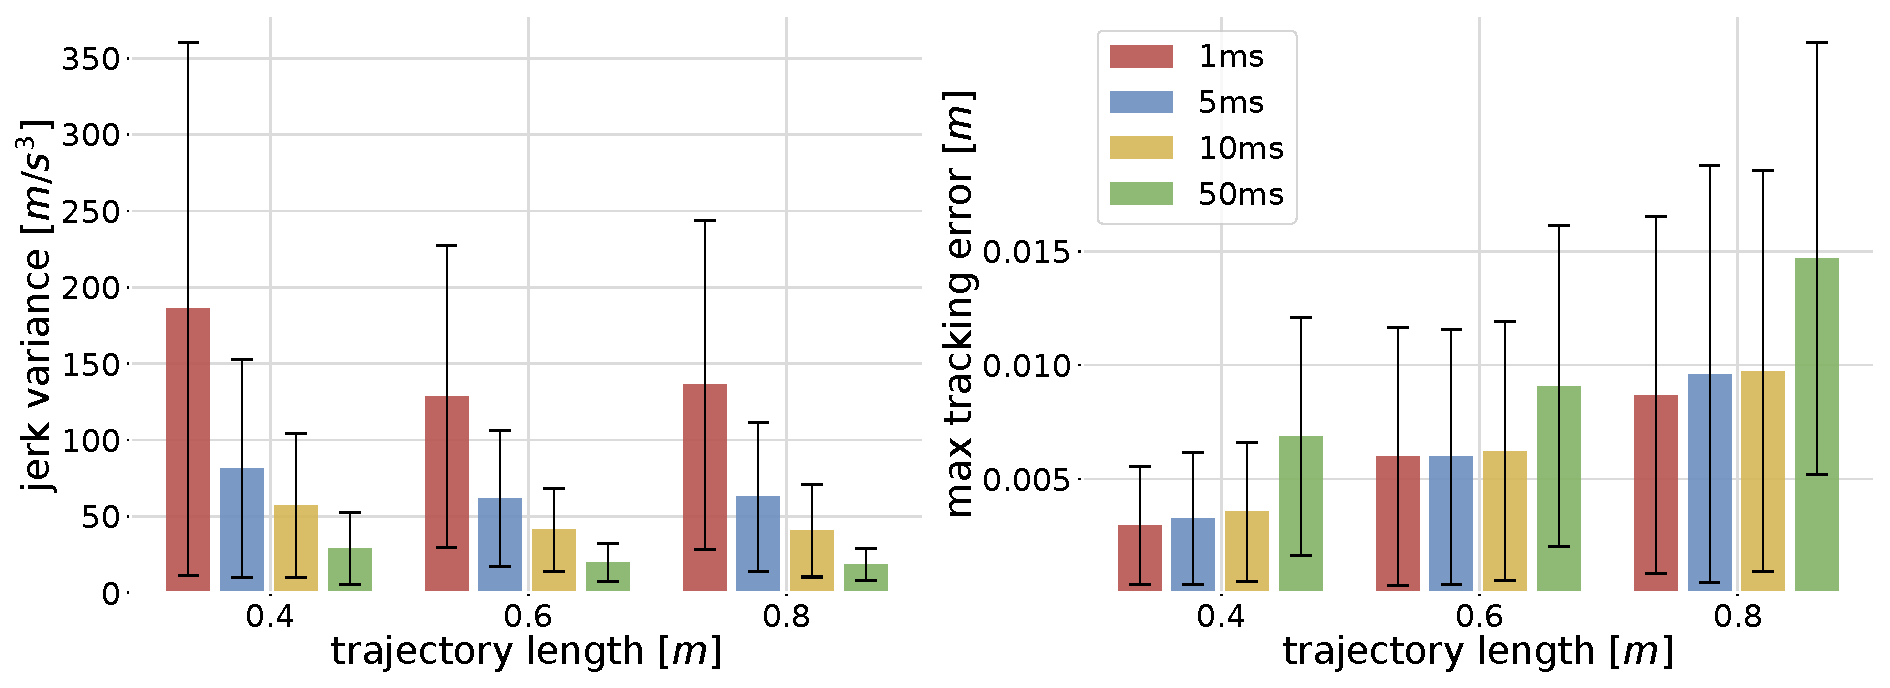
\includegraphics[width=\linewidth]{Papers/imgs/compensation_comp_oscillations.pdf}
    \caption{Plots showing the comparison of the jerk variance(left) and following error (right) of the proposed method with and without oscillation compensation, for trajectory lengths $d=0.4$, $0.6$ and $0.8m$. Means and variances are calculated over 100 random trajectories. }
    \label{fig:compensatiopn_comp_oscillations}
\end{figure}
In order to find the optimal down-sampling time $\Delta t_p$ an empirical study is conducted for 100 random trajectories with lengths $d=40cm$, $60cm$ and $80cm$ in the robots workspace. The experiments were conducted in simulation using a Franka Emika Panda robot, the implementation details are described in \Cref{ch:setup}. Four down sampling times were compared $\Delta t_p =1ms$, $5ms$, $10ms$ and $50ms$. For each executed trajectory the maximal deviation from the path and the \gls{cs} jerk variance is evaluated. 

\Cref{fig:compensatiopn_comp_oscillations} demonstrates an inverse proportionality between the down sampling time and the jerk variance. Additionally, it reveals that as the planning time step $\Delta t_p$ increases, there is a corresponding increase in the deviation from the desired path. Therefore, the choice of the appropriate planning time step $\Delta t_p$ implies making a trade-off between the two. In the case of this work, the planning step $\Delta t_p=10ms$ is chosen, resulting in a significant decrease in the jerk variance while having relatively low impact on the tracking error.



\section{Experimental setup}
\label{ch:setup}


All the experiments, both in simulation and in real world, are conducted on a Franka Emika Panda robot. The robot's kinematic limits in \gls{js} and the\gls{cs} are obtained from Franka Emika's official datasheet~\cite{frankadata}.  These values are publicly available\footnote{\label{note:topca_franka}Full datasheet available at: \url{https://frankaemika.github.io/docs/control_parameters.html}} and are listed in \Cref{tab:panda_limits_js} and \Cref{tab:franka_limits}.

\begin{table}[h!]
    \centering
    \begin{tabular}{|c|ccccccc|}
        \hline
        Limits & $q_0$ & $q_1$ & $q_2$ & $q_3$ & $q_4$ & $q_5$ & $q_6$ \\
        \hline
        $\dot{\bm{q}}_{max}$ $[{rad}/{s}]$ & 2.175 & 2.175 & 2.175 & 2.175 & 2.61 & 2.61 & 2.61 \\
        $\ddot{\bm{q}}_{max}$ $[{rad}/{s}^2]$ & 15 & 7.5 & 10 & 12.5 & 15 & 20 & 20 \\
        $\dddot{\bm{q}}_{max}$ $[{rad}/{s}^3]$ & 7500 & 3750 & 5000 & 6250 & 7500 & 10000 & 10000 \\
        \hline
    \end{tabular}
    \caption{Franka Emika Panda robot \gls{js} kinematic limits\footref{note:topca_franka}.}
    \label{tab:panda_limits_js}
\end{table}

	
\begin{table}[h]
    \centering
    \begin{tabular}{|c|cc|}
        \hline
        Limits & Translation & Orientation \\
        \hline
        $\dot{\bm{x}}_{max}$ & 1.7 $m/s$ & 2.5 $rad/s$ \\
        $\ddot{\bm{x}}_{max}$ & 13 $m/s^2$ & 25 $rad/s^{2}$\\
        $\dddot{\bm{x}}_{max}$ & 6500 $m/s^3$ & 12500 $rad/s^{3}$\\
        \hline
    \end{tabular}
    \caption{Franka Emika Panda robot \gls{cs} kinematic limits\footref{note:topca_franka}.}
    \label{tab:franka_limits}
\end{table}


\subsection{Robot control architecture}
\label{ch:qp}

\begin{figure}[!h]
    \centering
    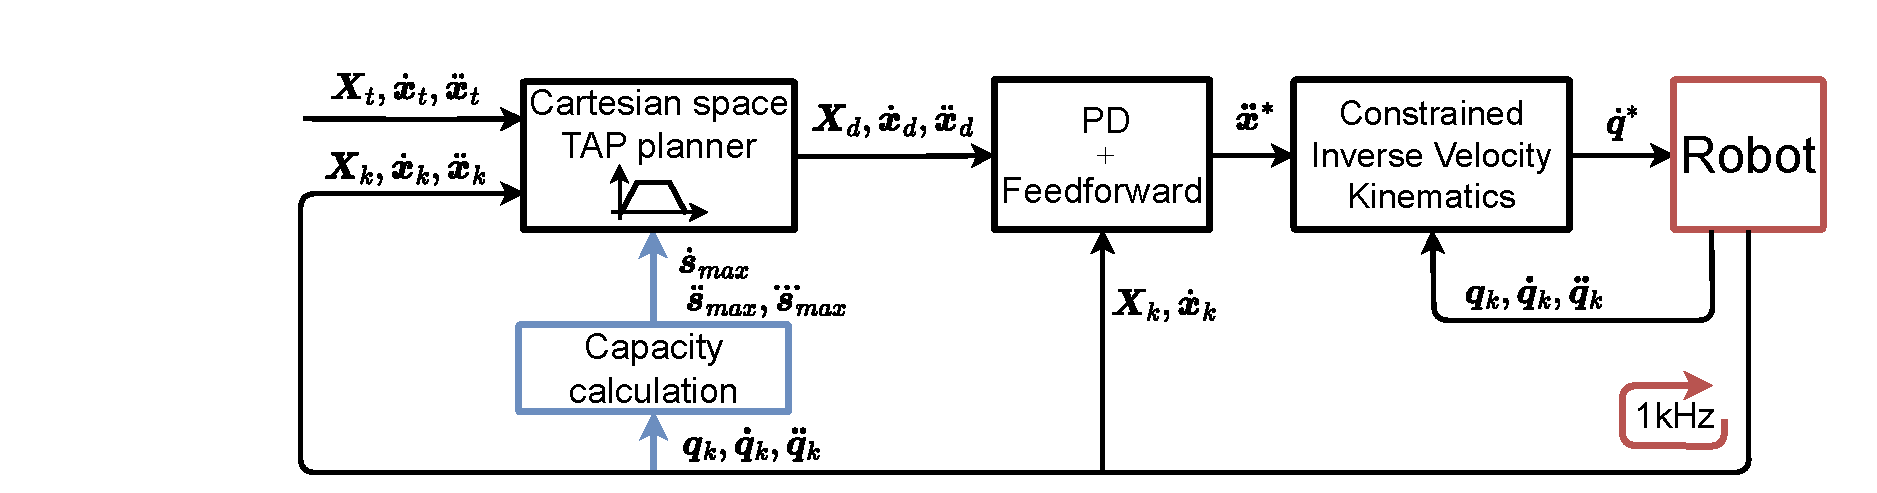
\includegraphics[trim=3cm 0 0 0, clip=true, width=\linewidth]{Papers/imgs/schema.pdf}
    \caption{Proposed method schematic overview in the context of the robot control, elements in blue present the extension of a standard \gls{cs} based \gls{tap} planning.}
    \label{fig:schema}
\end{figure}

The schematic diagram of the proposed approach within the robot control paradigm is shown on \Cref{fig:schema}. Given the robot's current state $\{\bm{q}_k,\dot{\bm{q}}_k,\ddot{\bm{q}}_k\}$ in step $k$, the approach first determines the robot's current \gls{cs} movement capacity in the path direction using the approach described in \Cref{ch:capacity_lp}, resulting in velocity $\dot{s}_{max}$, acceleration $\ddot{s}_{max}$ and jerk $\dddot{s}_{max}$ limits. Using the updated limits, the robot's current \gls{cs} state $X_k$,$\dot{\bm{x}}_k$,$\ddot{\bm{x}}_k$ and the target state $X_t$,$\dot{\bm{x}}_t$,$\ddot{\bm{x}}_t$,
the proposed method calculates the new optimal trajectory using \gls{tap} planning, as described in \Cref{ch:update_cap}.
Once the optimal \gls{tap} trajectory is found, desired states $X_{d}$,$\dot{\bm{x}}_d$,$\ddot{\bm{x}}_d$ are sent to the inverse velocity kinematics layer of the control architecture. 

In this work, the robot control strategy for real-time \gls{cs} trajectory following is formulated as a \gls{qp} and solved in each control loop. 
\begin{equation}
\begin{split}
    \ddot{\bm{q}}_{opt} = \arg \min_{\ddot{\bm{q}}}& \quad \overbrace{|| \dot{\bm{\nu}}^* - J(\bm{q}_k)\ddot{\bm{q}} - \dot{J}(\bm{q}_k,\dot{\bm{q}}_k)\dot{\bm{q}}_k ||^2}^{\text{trajectory tracking}} + \overbrace{\omega_r || \ddot{\bm{q}}_r - \ddot{\bm{q}} ||^2}^{\text{regularisation}} \\
    \text{s.t.} \quad \ddot{\bm{q}} &\in [\ddot{\bm{q}}_{ub}(\bm{q}_k,\dot{\bm{q}}_k,\ddot{\bm{q}}_k), ~\ddot{\bm{q}}_{lb}(\bm{q}_k,\dot{\bm{q}}_k,\ddot{\bm{q}}_k)]
\end{split}
\label{eq:qp_robot_control}
\end{equation}
where the $\bm{q}_k,\dot{\bm{q}}_k,\ddot{\bm{q}}_k\in\mathbb{R}^n$ is robot's current state, $J(\bm{q}_k)\in\mathbb{R}^{m\times m}$ and $\dot{J}(\bm{q}_k,\dot{\bm{q}}_k)\in\mathbb{R}^{m\times n}$ are the robot's state dependent jacobian matrix and its time derivative. The bounds of each of joint accelerations $\ddot{{q}}_{i,ub}$, $\ddot{{q}}_{i,lb}$ are calculated in a way to guarantee that the joint jerk $\dddot{\bm{q}}$, velocity $\dot{\bm{q}}$ and position $\bm{q}$ in the horizon $\delta t$ respect their limits. 
\begin{equation}
    \ddot{{q}}_{i,ub} = \min  \Big\{ \underbrace{\ddot{{q}}_{i,k} + \dddot{q}_{i,max}\delta t}_{\text{jerk}}, ~
    \underbrace{\ddot{{q}}_{i,max}}_{\text{acceleration}}, ~ 
    \underbrace{\frac{1}{\delta  t}(\dot{{q}}_{i,max} - \dot{{q}}_{i,k})}_{\text{velocity}}, ~
    \underbrace{\frac{2}{\delta  t^2}({{q}}_{i,max} - {{q}}_{i,k} - \dot{{q}}_{i,k}\delta  t )}_{\text{position}}
    \Big\}  
\label{eq:qp_limits}
\end{equation}
where the horizon $\delta t$ has to be chosen long enough to ensure constraints compatibility without leading to conservative behaviour~\cite{Prete2018}. Equation (\ref{eq:qp_limits}) shows the upper bound expression, the lower bound calculation is equivalent, and is obtained by substituting \textit{min} for \textit{max} and maximising instead of minimising.  The horizon $\delta t$ chosen for the experitments is 15ms. 

The optimisation problem  (\ref{eq:qp_robot_control}) consists in two tasks: trajectory tracking task and a secondary (regularisation) task.

\paragraph*{Trajectory following task} The trajectory following task is accomplished by following the desired \gls{cs} acceleration $\dot{\bm{\nu}}^*$. the control law formulated as a PD controller with a feed-forward term through the desired Cartesian acceleration $\dot{\bm{\nu}}^*$
\begin{equation}
\begin{split}
    \dot{\bm{\nu}}^* &= K_p \bm{e} + K_d(\dot{\bm{x}}_{d} - \dot{\bm{x}}_k) + \ddot{\bm{x}}_{d} \\
    \bm{e} &= \text{Ad}(X_k) \log(X_k^{-1}X_{d})\\
\end{split}
\end{equation}
$X_d$,$\dot{\bm{x}}_d$,$\ddot{\bm{x}}_d$ are the desired \gls{cs} pose, velocity and acceleration in the next step, while $X_{k}$ and $\dot{\bm{x}}_{k}$ are the measured \gls{cs} pose and velocity in current step $k$. $K_p,K_d\in \mathbb{R}^m$ are diagonal matrices containing the proportional and derivative gains. Vector $\bm{e}$ is the \gls{cs} pose error expressed in the world frame. 

Robot is controlled using the joint velocity commands which are calculated using an Euler backward numerical integration
\begin{equation}
\dot{\bm{q}}^*_{k+1} = \dot{\bm{q}}^*_{k} +  \ddot{\bm{q}}_{opt}\Delta t  
\end{equation}

In the experiments, the PD controller gains used are $$K_p=\text{diag}\big([170.0, 170.0, 170.0, 100.0, 100.0, 100.0]\big)$$ and $$K_d=\text{diag}\big([50.0, 50.0, 50.0, 30.0, 30.0, 30.0]\big)$$

\paragraph*{Regularisation task}  The robot's redundant degrees of freedom are used to dampen the movement in the trajectory null-space and keep the robot away from its joint limits. The regularisation task is expressed through the joint acceleration $\ddot{\bm{q}}_r$
\begin{equation}
    \ddot{\bm{q}}_r = k_{rp}(\bm{q}_{r} - \bm{q}) - k_{rd}\dot{\bm{q}}
\end{equation}
where $k_{rp}$ and $k_{rd}$ are scalar gains and $\bm{q}_{r}$ is the initial robot pose at the center of all the joint ranges.
$$
\bm{q}_r = \frac{\bm{q}_{max}+\bm{q}_{min}}{2}
$$
The secondary task gains used are $k_{rp}=5 s^{-2}$ and $k_{rd}=2\sqrt{k_{rd}}s^{-1}$, while secondary task weight is $\omega_r=1e^{-5}$.


\subsection{Software implementation details}
The simulation experiments used for the comparative studies are implemented in Python
using open-source implementations of TOPP-RA \cite{Pham2018} and \gls{tap} planning implementation within \codet{Ruckig} library \cite{ruckig}. The code used for the simulation experiments is open-source and can be found on GitLab\footnote{\url{https://gitlab.inria.fr/auctus-team/people/antunskuric/papers/catp}}.

For the mock-up experiment, the real-time execution of the proposed method is implemented in C++. The \gls{tap} planning is implemented using the open-source library \codet{Ruckig} \cite{ruckig}, while the efficient \gls{lp} solver used for real-time \gls{cs} limit calculation is GLPK \cite{glpk}. All the software components are integrated using \gls{ros}.

Additionally, both simulation and real world experiments used robot rigid body dynamics simulation implemented using the open-source library \codet{Pinocchio} \cite{pinocchio2021}. 



\section{Comparative study}
\label{ch:comp_study}
A simulation based comparative study is conducted to evaluate the performance of the proposed method against well known time-optimal planning algorithms. The proposed algorithm is first compared to the state of the art time-optimal \gls{js} planning method called TOPP-RA \cite{Pham2018}. Furthermore the proposed algorithm is compared against the \gls{tap} planning with fixed \gls{cs} limits provided by the manufacturer.

\subsection{Benchmarking against time-optimal Joint space planning}

\begin{figure}[!t]
    \centering
    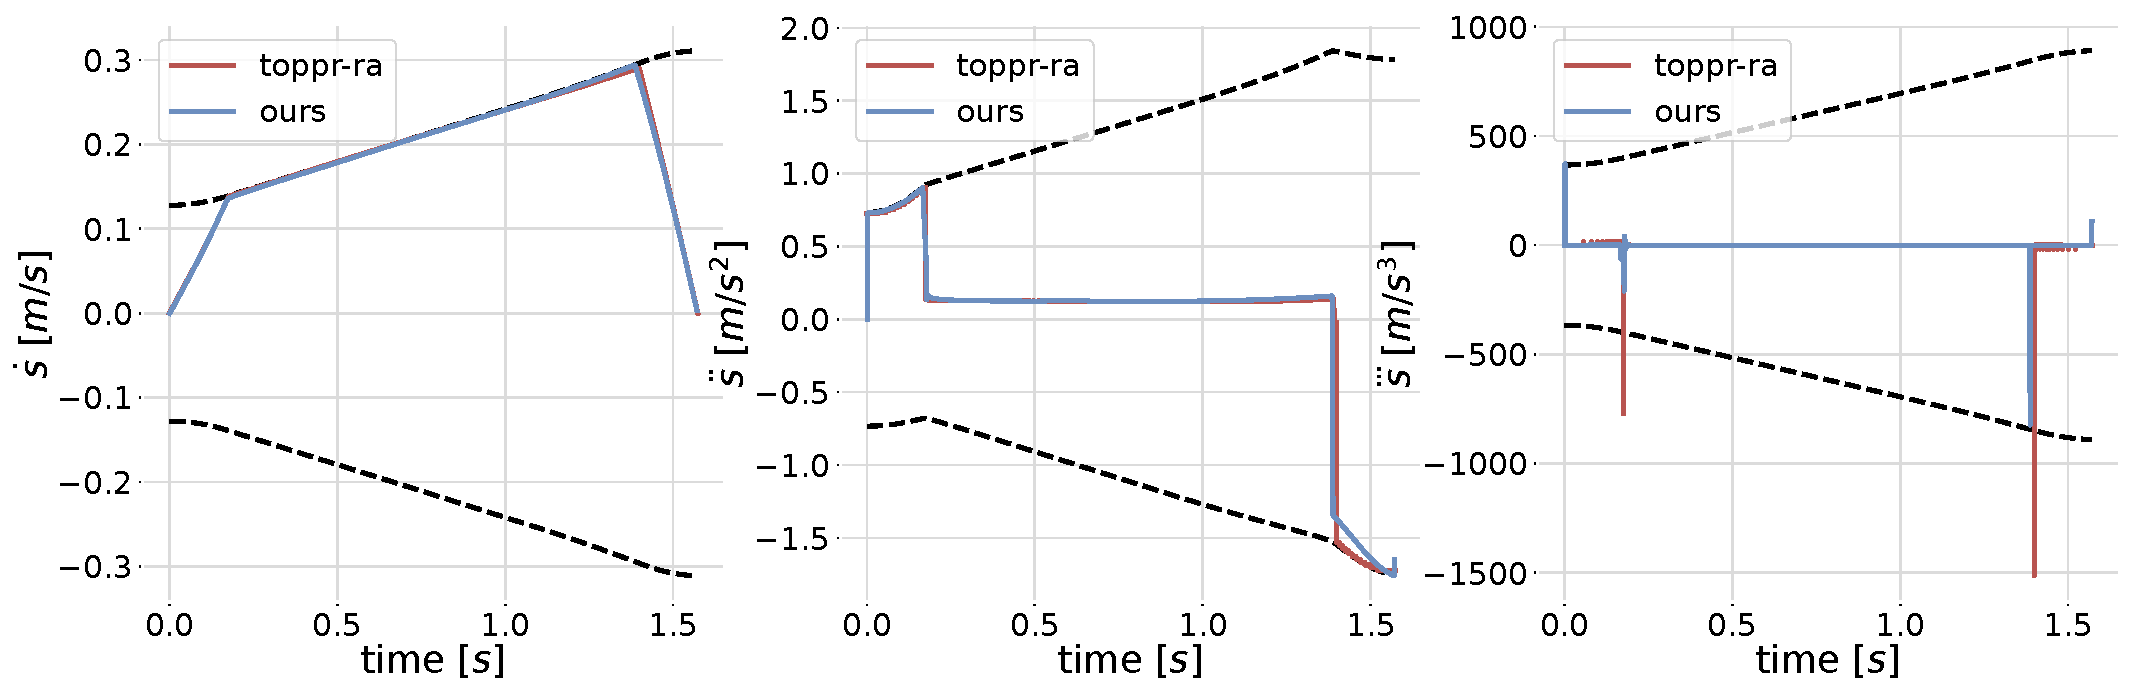
\includegraphics[width=\linewidth]{Papers/imgs/ruckig_toppra_comp1679478306.pdf}
    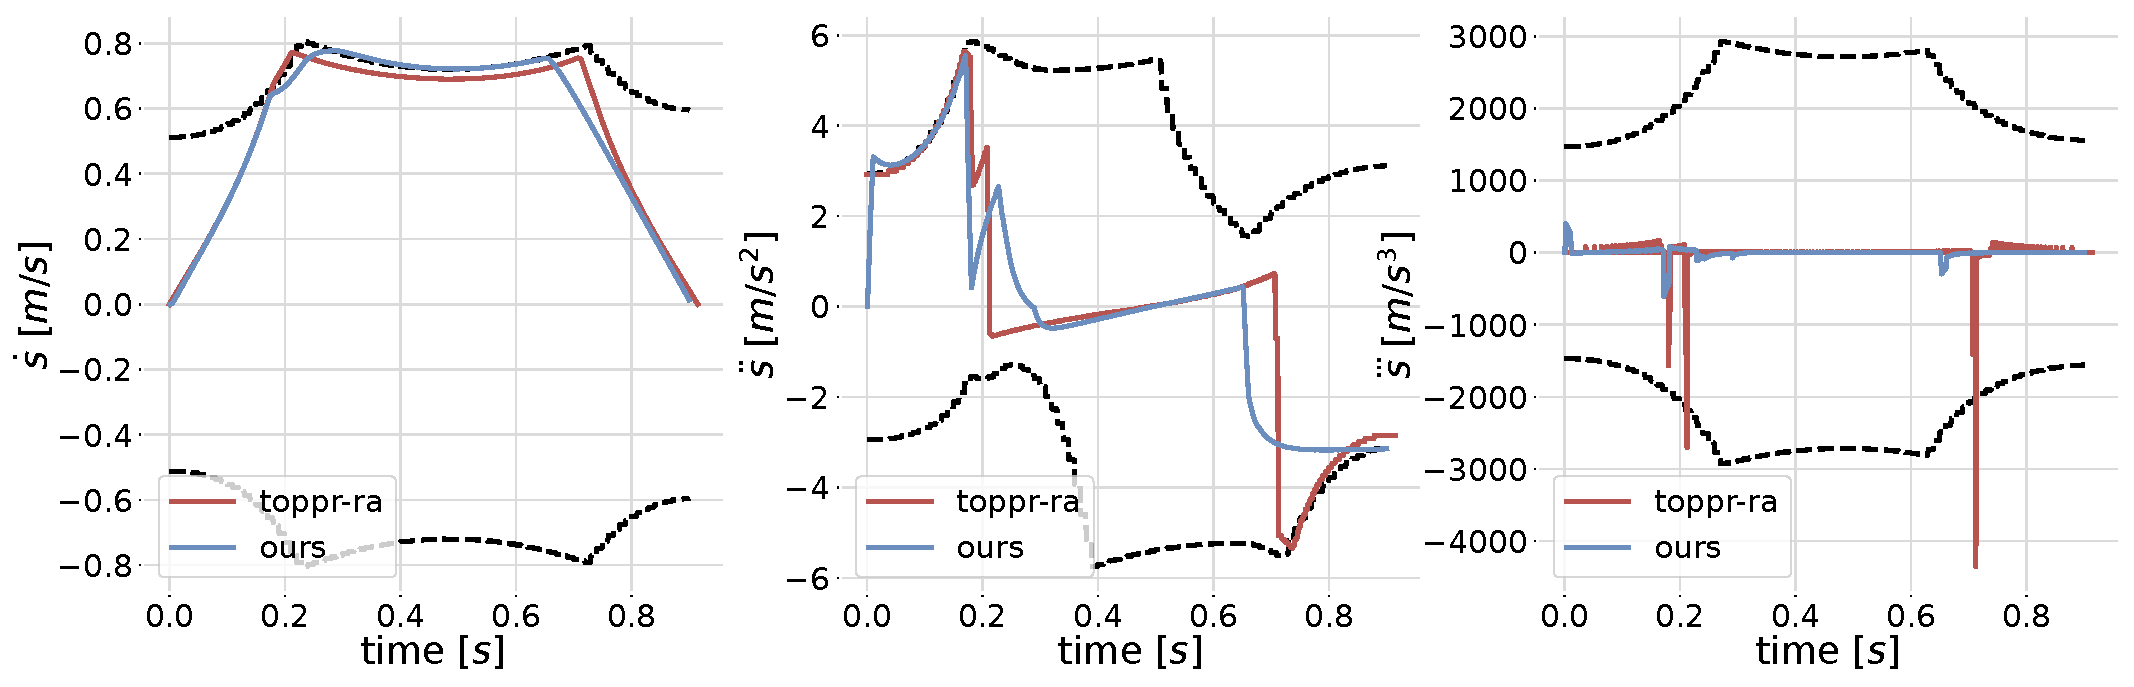
\includegraphics[width=\linewidth]{Papers/imgs/ruckig_toppra_comp1681374566.pdf}
    \caption{The plots show the comparison of the path velocity, acceleration and jerk, generated by the proposed approach (blue) and TOPP-RA(red), for two different trajectories (up and down). The dashed lines show the robot's movement limits in the trajectory direction calculated using the proposed method, described in \Cref{ch:capacity_lp}. }
    \label{fig:comparison_trajectory}
\end{figure}

In order to evaluate the performance of the trajectories found and executed by the proposed \gls{cs} planning approach, it is compared against the state-of-the art time-optimal \gls{js} planning algorithm TOPP-RA \cite{Pham2018}. TOPP-RA takes in consideration the robot's \gls{js} velocity and acceleration limits and plans for the minimum time \gls{js} trajectories.
Both algorithms are run on a set of 1000 random straight line trajectories (with random fixed orientation), ranging in length from $d=10cm$ to $1m$. The goal of this experiment is to compare the generated trajectory profiles of TOPP-RA and the proposed approach as well as their execution times, in order to asses the tome optimally of the proposed real-time planning approach. 

TOPP-RA's limitation however is that it cannot deal with \gls{cs} trajectories directly and it requires an additional step of finding the \gls{js} path corresponding to the \gls{cs} path. For TOPP-RA, the full \gls{js} path is determined by sampling the \gls{cs} path $\mathscr{P}(s)$ into the set of way-points $X_{w,i}$ and finding the inverse kinematic solution $\bm{q}_{w,i}$ for each one of them. To ensure the \gls{js} path continuity, the inverse kinematics solution $\bm{q}_{w,n+1}$ at the way-point $X_{w,n+1}$ is taken as the one closest to the joint configuration $\bm{q}_{w,n}$ in the previous way-point $X_{w,n}$. The distance between the way-points used in these experiments is $5cm$. 

Both approaches are tested using 50\% of the robot's \gls{js} velocity, acceleration and jerk capacity $\alpha_v\!=\!\alpha_a\!=\!\alpha_j = 0.5$. 

% \todo[inline]{argue about the 5cm waypoint and 50\% capacity.}


\subsubsection*{Results} The comparison of the planned velocity, acceleration and jerk profiles for two trajectories are shown on \Cref{fig:comparison_trajectory}. It can be seen that both methods find similar time profiles for all the path variables, indicating the effectiveness of the proposed approach. Moreover, even though TOPP-RA plans entirely in \gls{js} it s\gls{cs} trajectory respects the \gls{cs} velocity and acceleration limits calculated by the proposed method, demonstrating the accuracy of limit calculations. Additionally, TOPP-RA does not limit the jerk which can be seen on the jerk plots in \Cref{fig:comparison_trajectory}.

Additionally, the influence of the overshoot compensation strategy can be observed in the second (bottom) trajectory. The proposed approach starts braking earlier and does not use the full braking capacity of the robot. The resulting trajectory does not have an overshoot, even though the robot's braking capacity decreases significantly towards the end of the trajectory. This demonstrates the effectiveness of the proposed strategy in reducing overshoot while not significantly increasing the execution time.

% \todo[inline]{Something like that}
The trajectory execution time comparison is presented in \Cref{fig:comparison_time}. The figure shows that the proposed method has a comparable execution time for all tested trajectory lengths. Interestingly, for lengths over $40cm$, our approach is even faster than TOPP-RA. This can be attributed to the fact that our method takes a different \gls{js} path than TOPP-RA, which in some cases might be more optimal than the one calculated in advance. 
This effect is more present for longer trajectories, where taking the \gls{js} path the closest to the initial joint configuration might not be the most optimal criteria. 

% \todo[inline]{say that this is not planned and that this happens more for the long trajectories because the chance that the toppra's \gls{js} trajectory is not optimal is higher for them than for the shorter ones.}

\begin{figure}[!t]
    \centering
    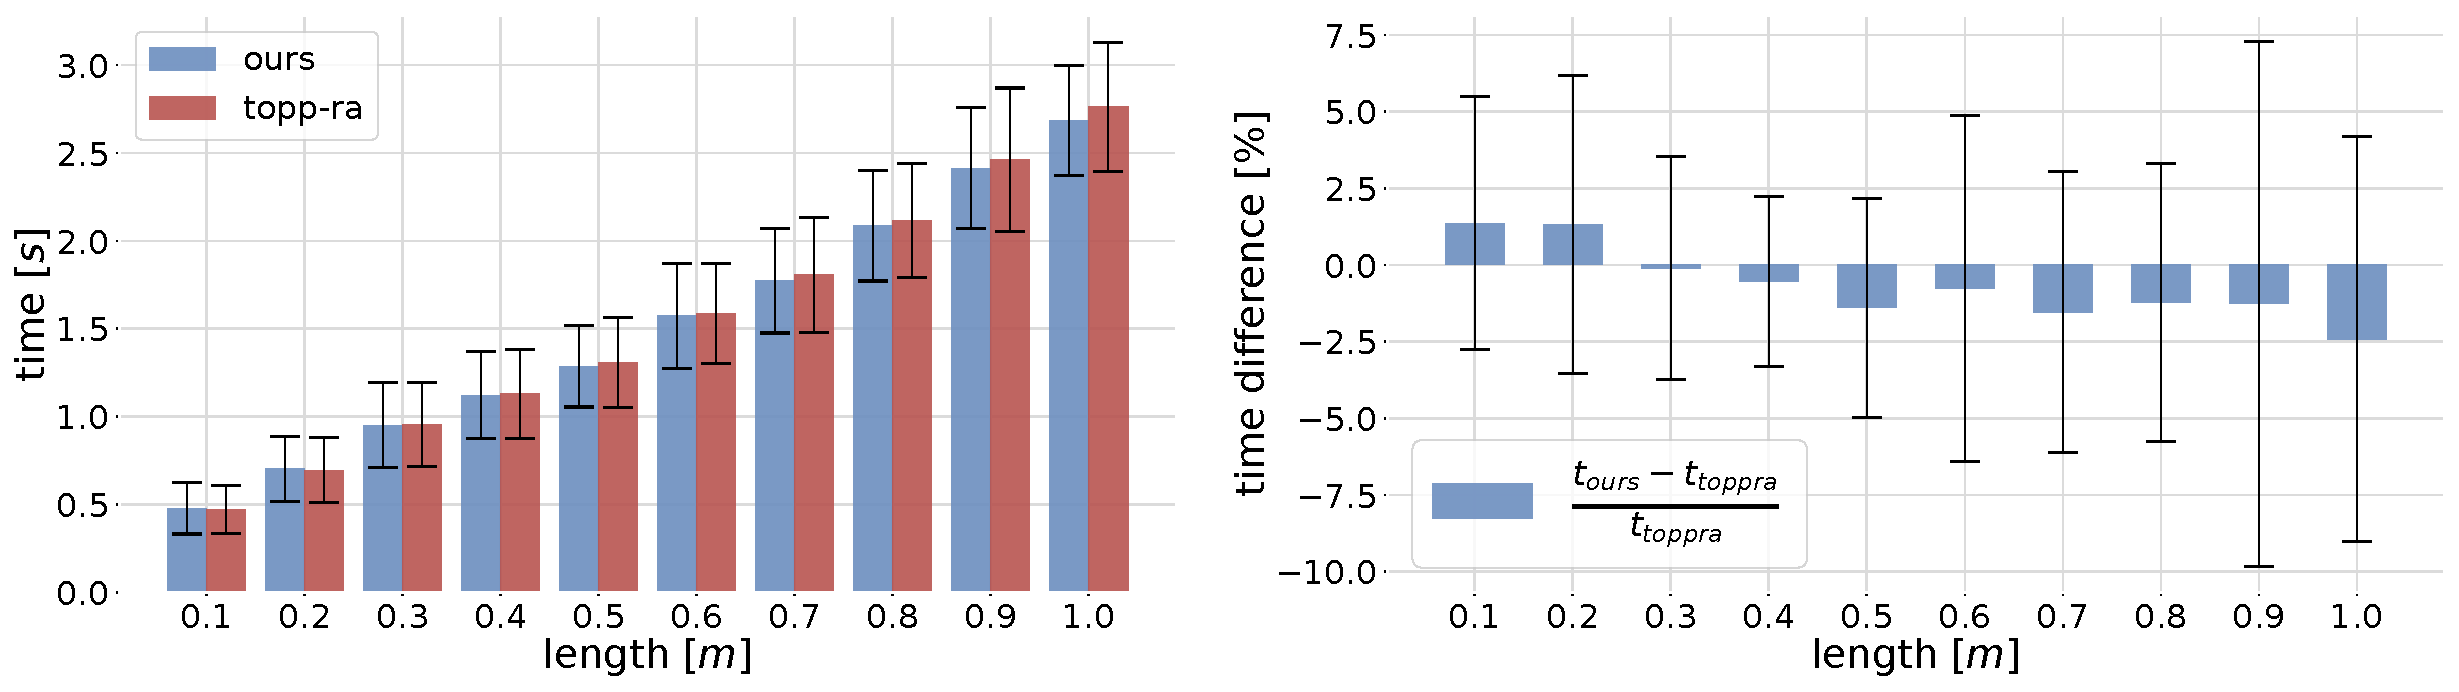
\includegraphics[width=\linewidth]{Papers/imgs/toppra_ruckig_time_comp.pdf}
    \caption{Plots showing the comparison of the trajectory execution time of the proposed method with TOPP-RA, for trajectory lengths ranging from $d=0.1$ to $1m$. Left graph shows the comparison of the execution time, while the graph on the right shows the difference in execution time in a form of percentage. Means and variances are calculated over 100 random trajectories.}
    \label{fig:comparison_time}
\end{figure}


\subsection{Benchmarking against time-optimal Cartesian space planning}

The proposed adaptive approach is further compared to the standard \gls{tap} trajectory planning using fixed \gls{cs} kinematic limits. The \gls{cs} limits for the Franka Emika panda robot are taken from the standard datasheet \cite{frankadata}, as given in \Cref{tab:franka_limits}.

The approaches are compared over 100 random robot straight line trajectories (with random fixed orientation), in the robot's workspace, with a fixed length of $d=50cm$. The performance of the two approaches is compared for different scaling levels $\alpha$, starting at 10\% ($\alpha$=0.1) of robot's capacity and going to 90\% ($\alpha$=0.9). The scaling strategy is chosen to be equal for velocity, acceleration and jerk $\alpha\!=\!\alpha_v\!=\!\alpha_a\!=\!\alpha_j$. 

The implementation of the \gls{tap} trajectory generator for both approaches is done using the open-source library \codet{ruckig} \cite{ruckig}. The robot control strategy implemented for trajectory following is the same for both approaches as detailed in the \Cref{ch:qp}.

\subsubsection*{Results} 
In \Cref{fig:comp_fixed_cs}, the results of a comparative study between the proposed method and the \gls{tap} planning method with fixed \gls{cs} limits are presented. Both methods show a linear relationship between the tracking error and the ratio of capacity used ($\alpha$), however the proposed approach has significantly lower mean errors and variances for same values $\alpha$. This can be attributed, in part, to the overestimated \gls{cs} limits (\Cref{tab:franka_limits}) provided by the manufacturer for the Panda robot, see \Cref{fig:comp_cube_poly}. Due to this overestimation, the planned \gls{tap} trajectories, depending on the path direction in robot's workspace, can become infeasible and induce large tracking errors. This is particularly apparent when using larger percentage of the robot's movement capacity. \Cref{fig:comp_fixed_cs} (on the left) shows that the average tracking error for $\alpha \geq 0.7$ is larger than $10cm$ (while the length of the trajectory is $50cm$).

\Cref{fig:comp_fixed_cs} further shows that using 30\% of the manufacturer's \gls{cs} limits (i.e., $\alpha$=0.3) results in a tracking error of around 1.2cm, which is higher than any of the mean errors achieved by the proposed method for all tested values of $\alpha$.
While for $\alpha$=0.3, the fixed \gls{cs} planning has the execution time of 1.1 seconds, the proposed method has lower execution time for all $\alpha\geq0.7$. 
These results therefore confirm that when it comes to planning for highly dynamical trajectories, taking in consideration robot's true movement capacity results in faster and more precise movements. 


\begin{figure}[!h]
    \centering
    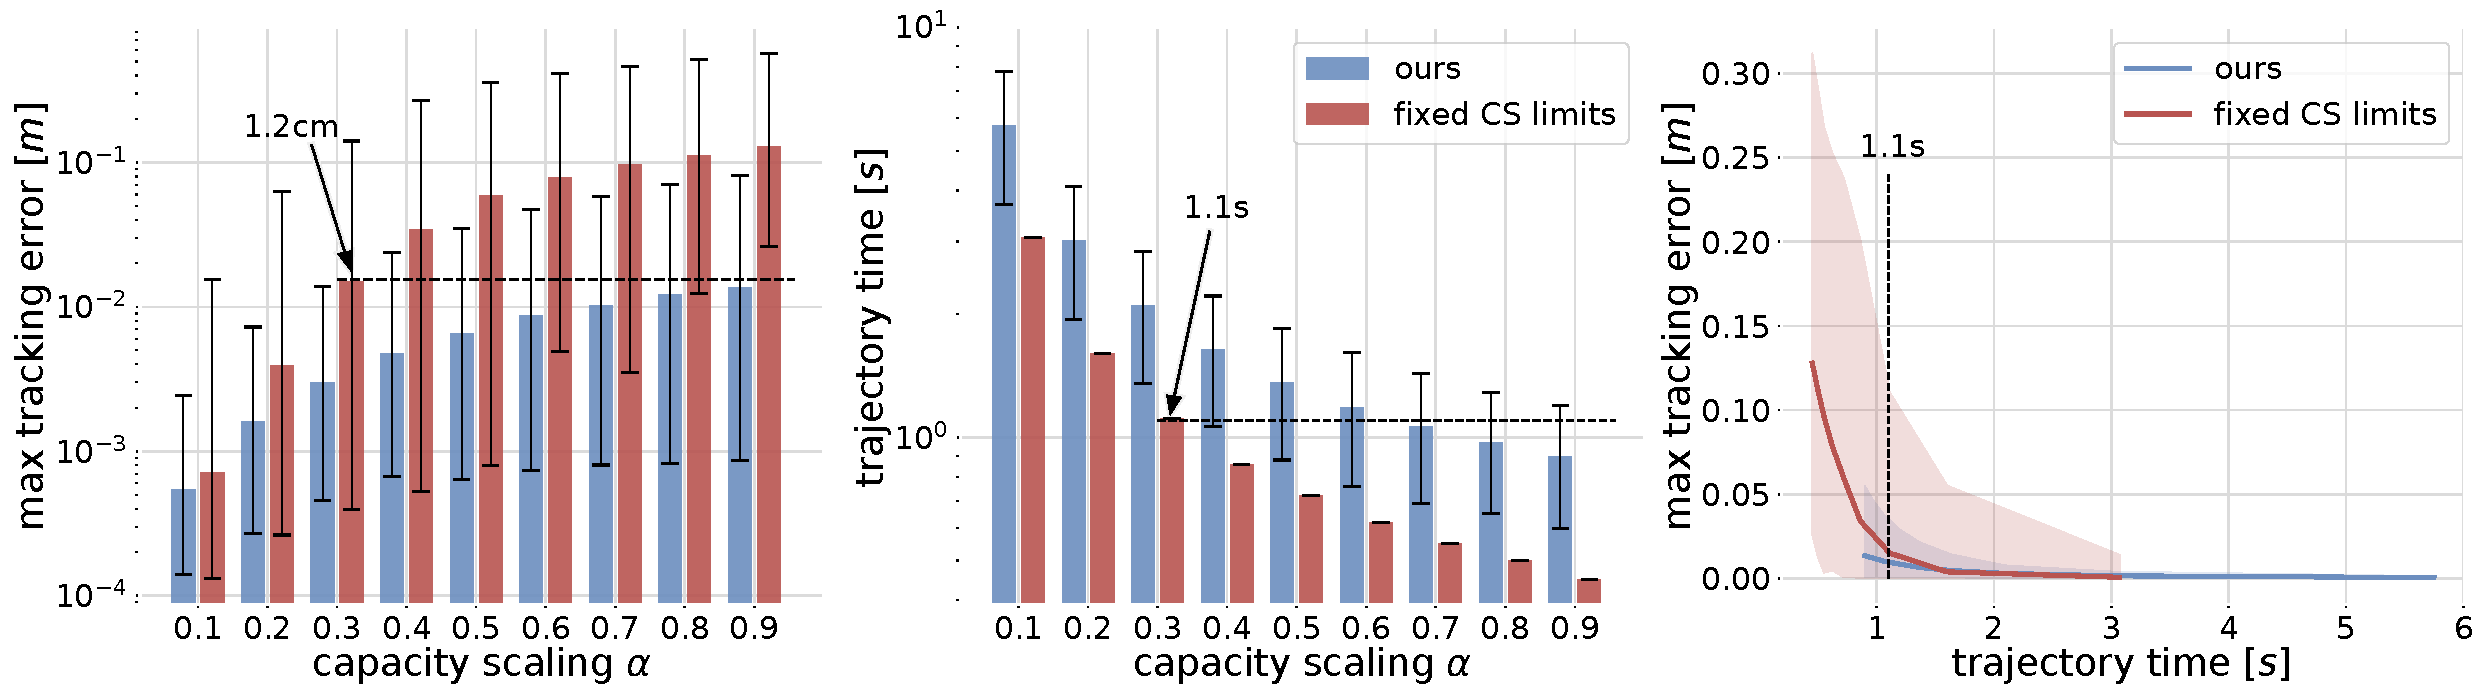
\includegraphics[width=\linewidth]{Papers/imgs/comparison_fixed_cs.pdf}
    \caption{Result of the benchmarking experiment comparing the fixed \gls{cs} planning approach (red) to the proposed method (blue). The graph on the left shows comparison of the max tracking error with respect to the ratio of the capacity $\alpha$ used while the graph in the middle shows the trajectory execution time comparison. The graph on the right unites the two graphs on the left in order to show the relation of the trajectory execution time against the max tracking error. Means and variances are calculated on 100 random robot trajectories. }
    \label{fig:comp_fixed_cs}
\end{figure}


% \begin{figure*}[!t]
%     \centering
%     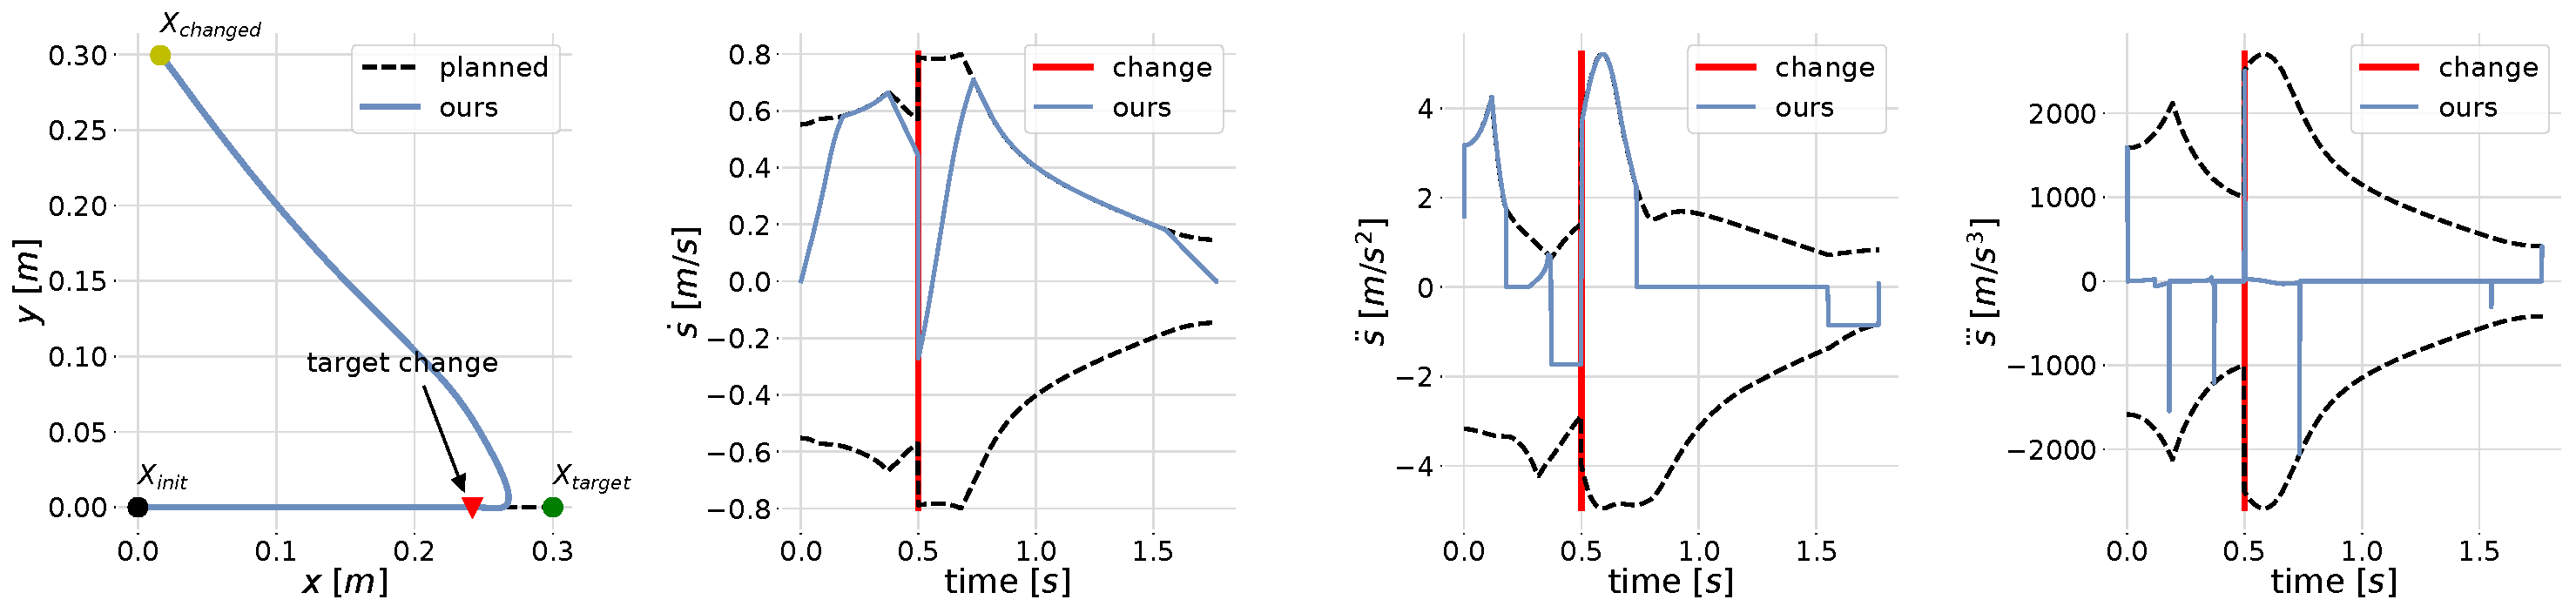
\includegraphics[width=\linewidth]{Papers/imgs/ruckig_plots_change_aio1680176621.pdf}
%     \caption{Write this}
%     \label{fig:change target}
% \end{figure*}



\section{Mock-up experiment: Collaborative waste sorting}
\label{ch:experiment_mockup}
% \begin{figure*}[!t]
%     \centering
%     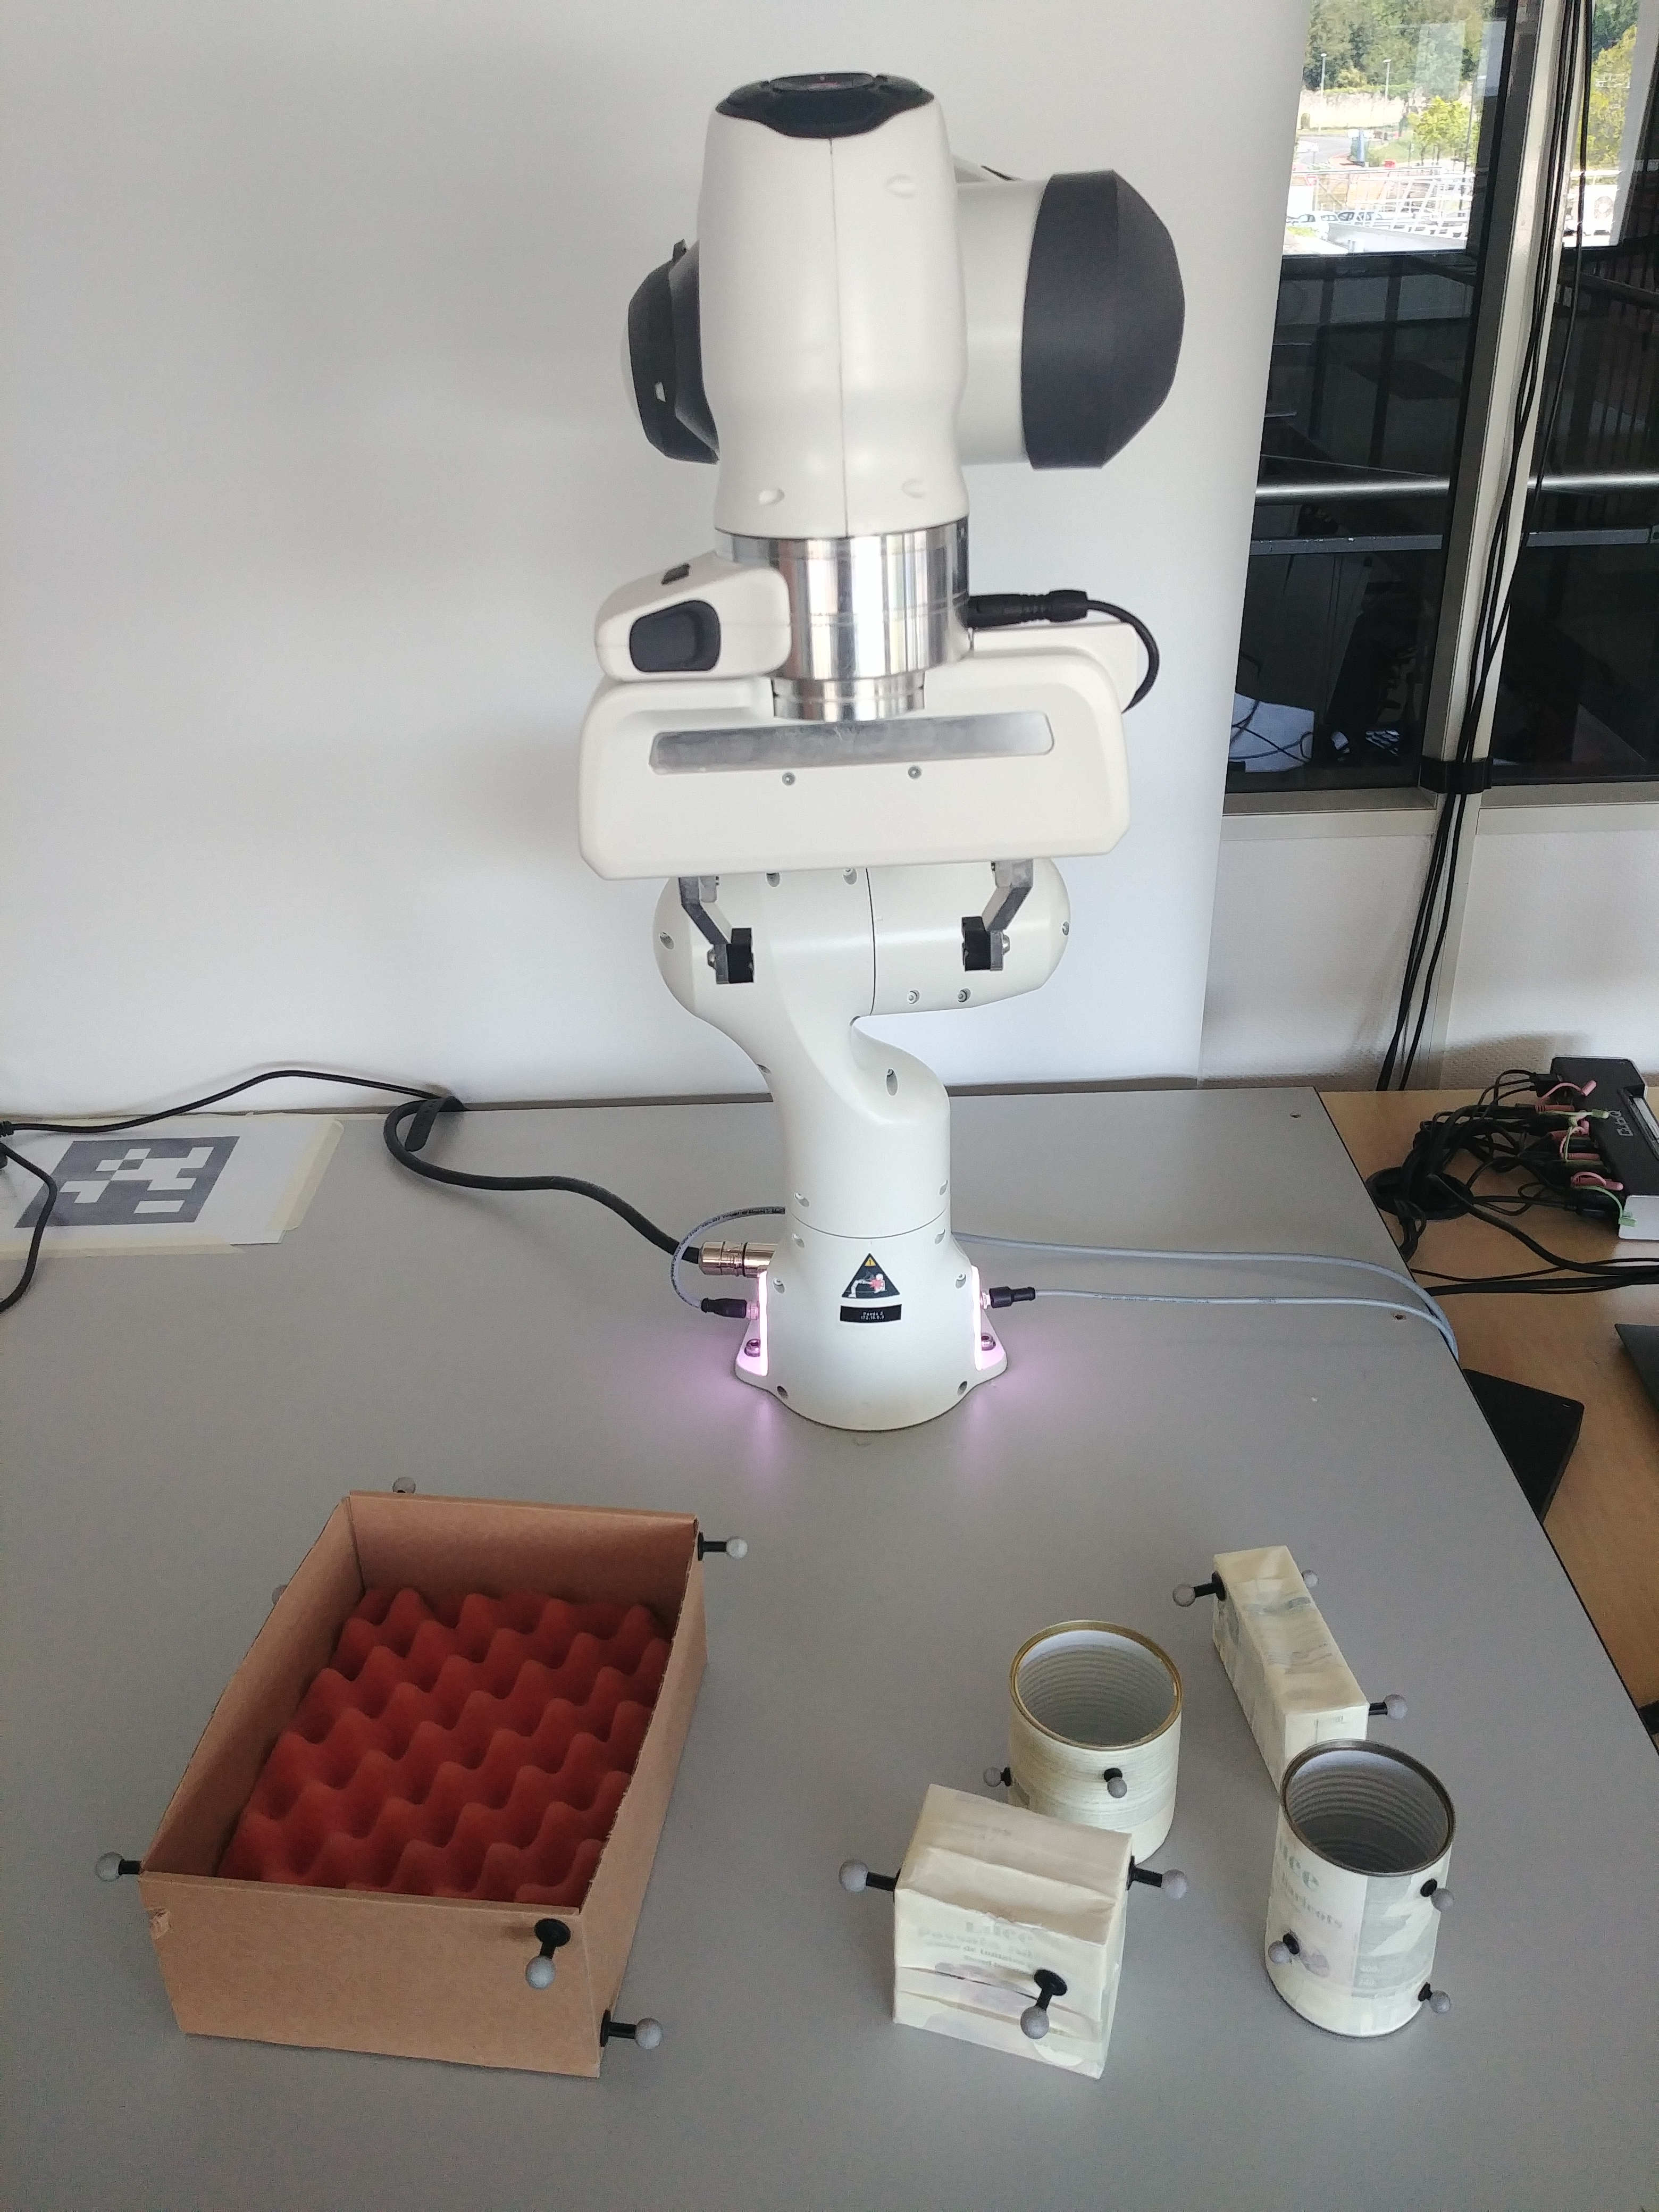
\includegraphics[width=0.26\linewidth]{Papers/imgs/setup.jpg}   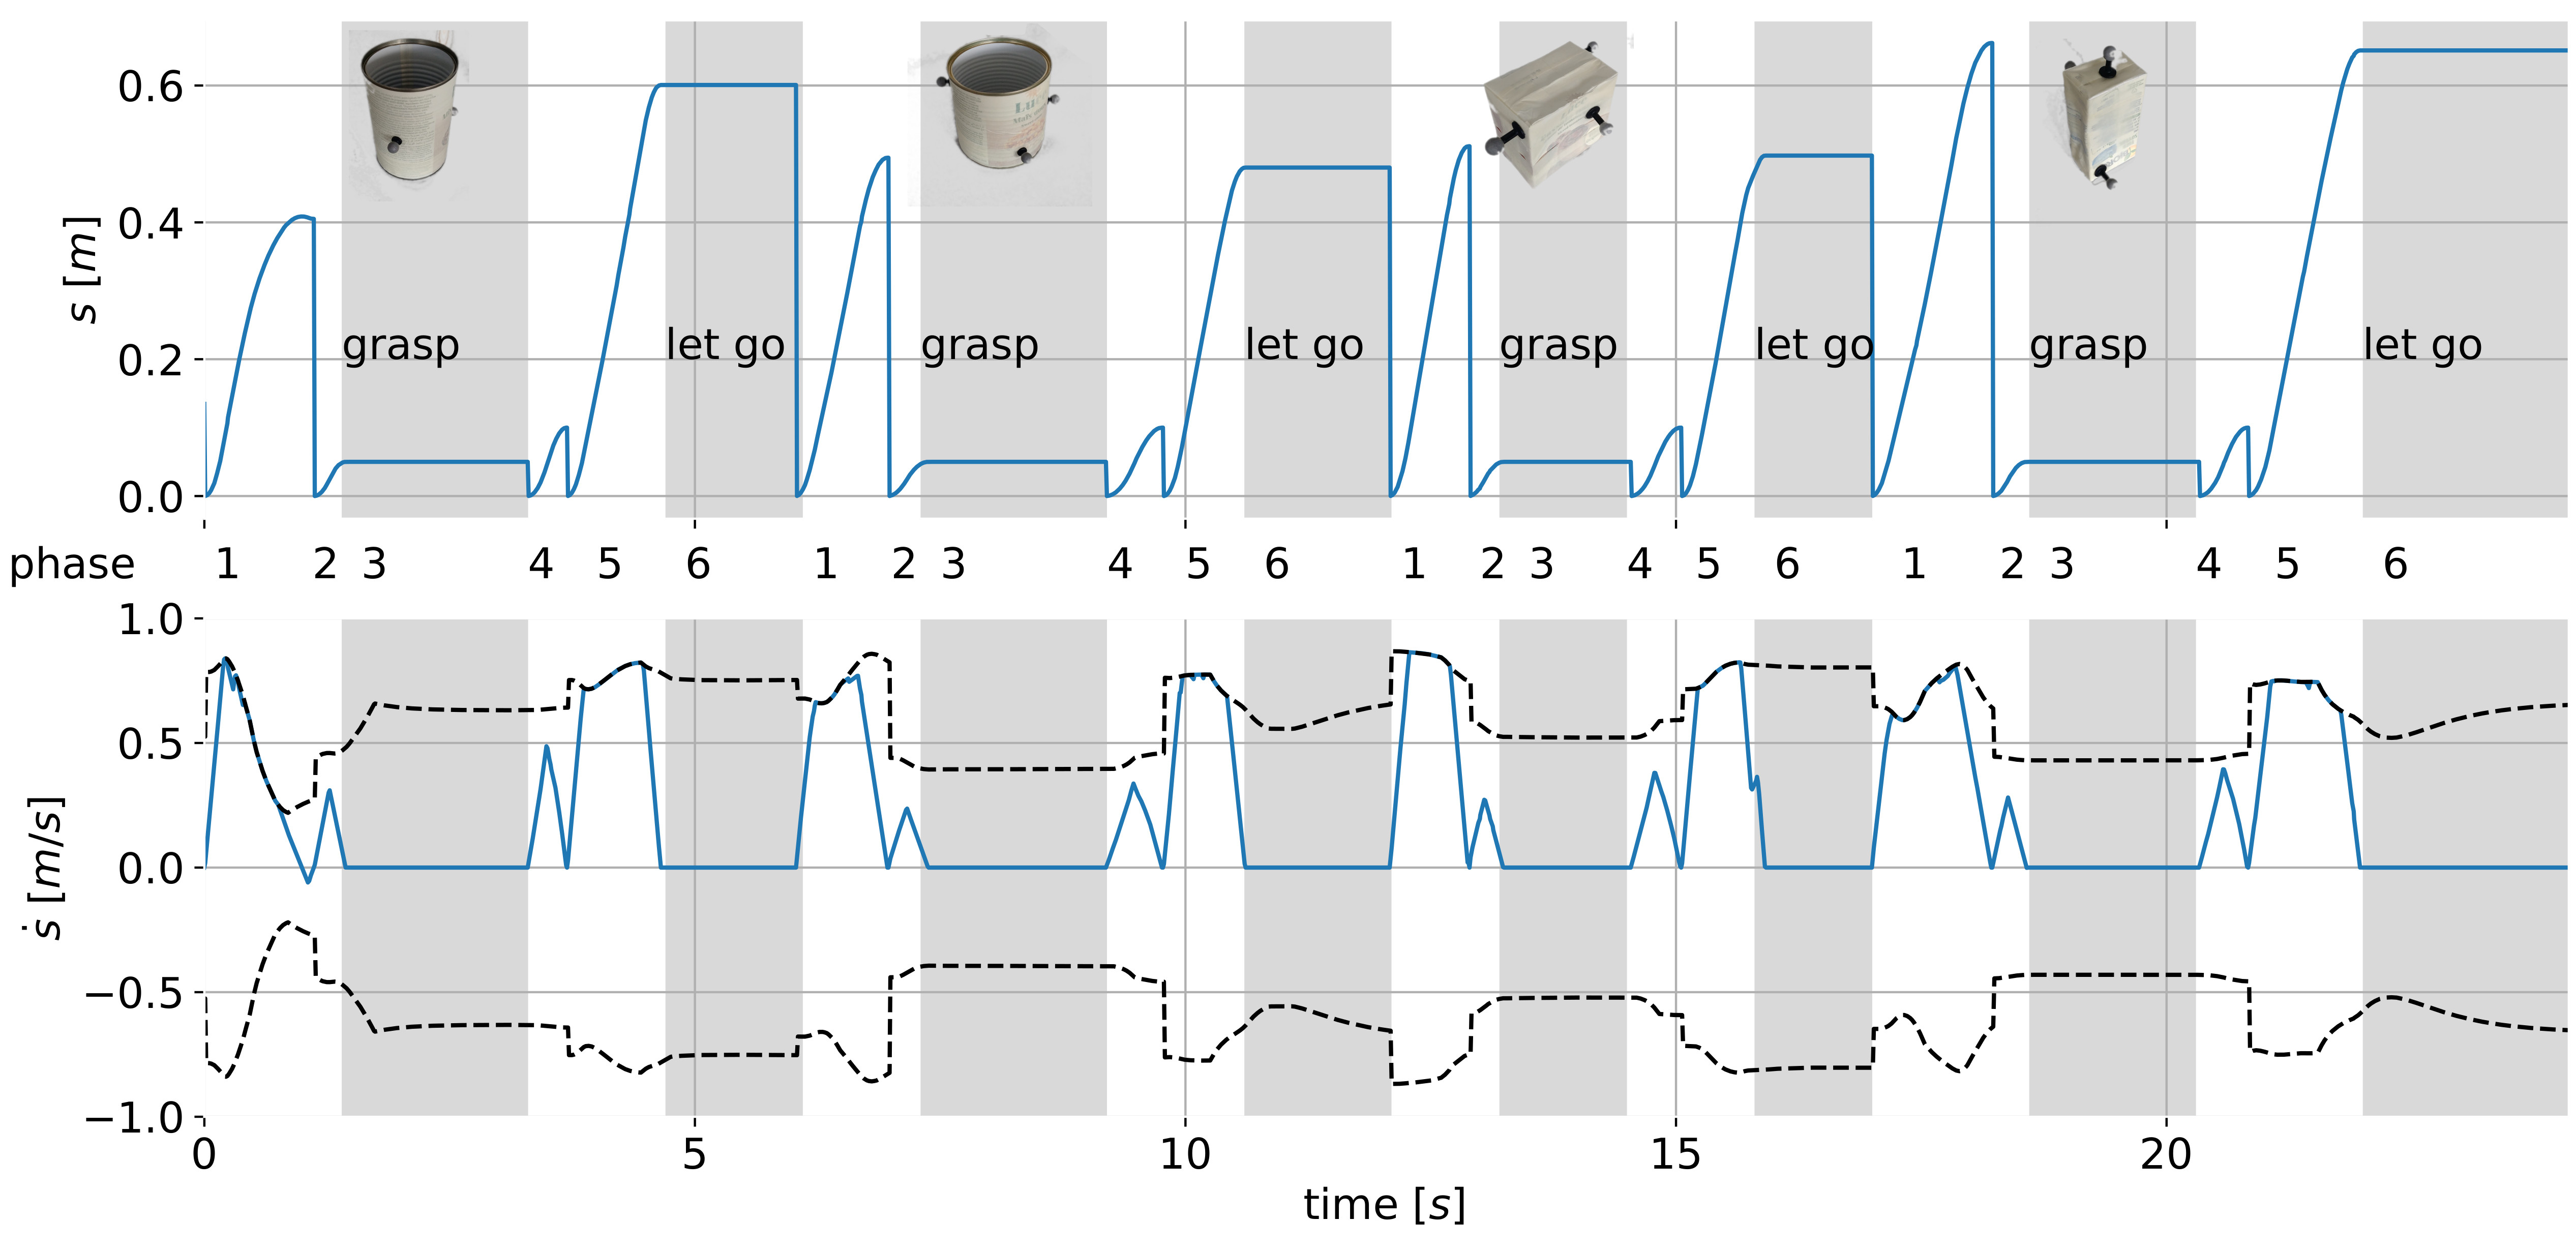
\includegraphics[width=0.73\linewidth]{Papers/imgs/experiment_main.jpg}
%     \caption{Write this}
%     \label{fig:setup}
% \end{figure*}

Waste recycling is an important tool for addressing the ecological issue of accumulating humanities waste. One of its  crucial parts is the waste sorting procedure, where the recyclable materials are extracted from the regular waste and prepared for the recycling process. Robotics and computer vision technologies have a great potential to improve the waste processing efficiency and increase its volume \cite{Koskinopoulou2021}. 
However, waste sorting is a highly dynamic and unstructured environment, presenting many challenges to potential robotised solutions. To be viable, waste sorting robots need to be able to operate at high speeds, where they use pick-and-place or pick-and-toss \cite{Hassan2022} techniques to sort the waste in different material groups. Therefore, one of the key challenges for building such systems is producing efficient and reactive movement generation techniques. 

Several robotic solutions have been proposed in the literature to address waste sorting tasks \cite{SARC2019}, such as \textit{Zenrobotics Fast picker}\footnote{Zenrobotics Fast picker: \url{https://zenrobotics.com/de/}} or \textit{SELMA}\footnote{SELMA: \url{https://www.opteknik.se}} . However, these solutions are based on expensive industrial robots and are only viable for large scale recycling facilities.

In this work, we propose a mock-up interactive (collaborative) scenario for waste sorting that leverages the proposed real-time trajectory planning method in order to create fast and adaptable robot movement. 

In the experiment, a human operator is introducing different waste items at the sorting workstation, where the robot is placed. The operator can introduce the waste items in any time and order, as well as modify their position and orientation on the table. The operator can do the same with the sorting buckets, the bins in which the sorted items are placed. The robot's job is to pick all the waste items and place them in the appropriate sorting buckets as fast as possible.

Waste items (two cans and two cartons), as well as the buckets, are tracked in real-time using a motion capture system \textit{Optitrack}. In order to efficiently and robustly sort the waste, object manipulation procedure is divided in 6 phases.
\begin{enumerate}
    \item Position the gripper 5cm above the object with the appropriate orientation
    \item Lower the gripper to the object
    \item Close the gripper
    \item Rise the object 10cm
    \item Transport the object to the appropriate bucket
    \item Release the object
\end{enumerate}

Robot control architecture, as described in \Cref{ch:qp}, and the proposed real-time planning approach are implemented in 
programming language C++, using \gls{ros} framework, and run in real-time at the frequency of 1kHz. For this experiment, 60\% of robot's capacity is used ($\alpha$=0.6) in order to keep the tracking error under 1cm, as shown on \Cref{fig:comp_fixed_cs}.
The experiment is available in a form of accompanying video\footnote{Video: \url{https://www.youtube.com/watch?v=BHGipnKNOfA}}.

\qrimg{qrcodes/waste.png}{https://www.youtube.com/watch?v=BHGipnKNOfA}{Video}
\afterpage{
\begin{landscape}
\begin{figure*}[!t]
    \centering
    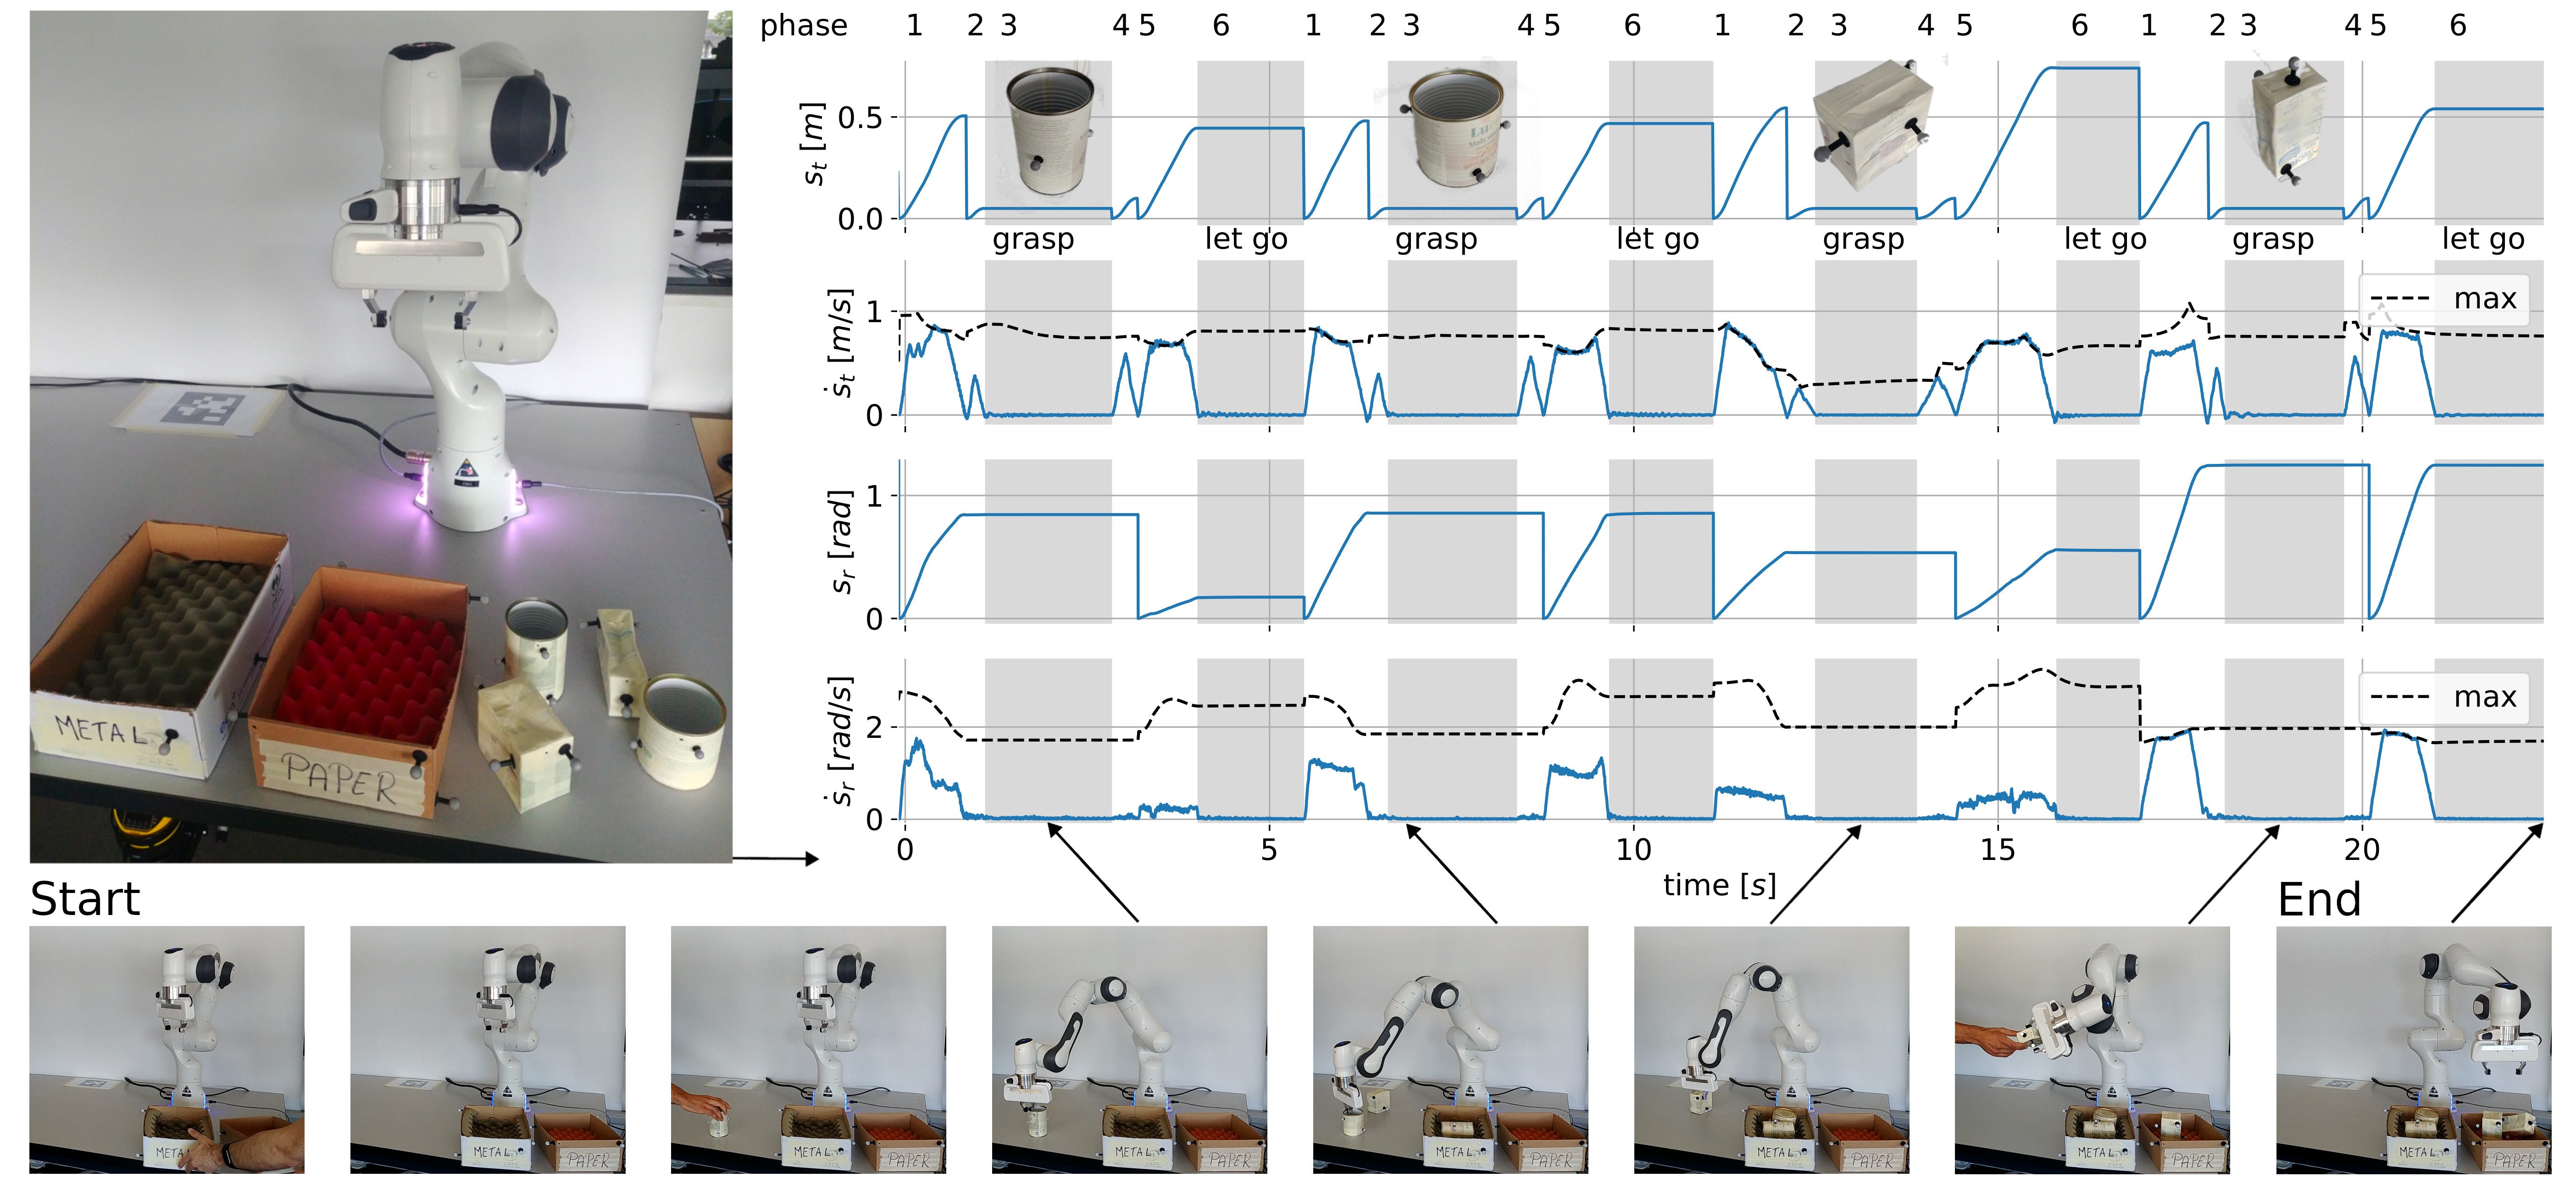
\includegraphics[width=\linewidth]{Papers/imgs/experiment_main_v2.3.jpg}   
    \caption{Figure on the left shows the experimental setup of the mock-up waste sorting experiment. The robot used in the experiments is a Franka Emika Panda robot. The experiment uses six objects: two cans, two cartons and two sorting bins, all tracked in real time using Motion capture system Optitrack. The images on the bottom show several moments of the experiment, while the plot (up right) shows the time evolution of the real-time executed trajectories. The plot shows the position $s_t$ and orientation $s_r$ path evolution in time as well as translation $\dot{s}_t$ and rotation $\dot{s}_r$ velocity on the path and their calculated maximal values (dotted lines).  In the experiment, the operator first brings the sorting bins to the robot workstation, then introduces the waste objects to the robot with unknown positions and orientations. Robot plans and executes in real-time the trajectories necessary in order to place, as fast as possible, the objects into the appropriate sorting bin.}
    \label{fig:setup}
\end{figure*}
\end{landscape}
}
\Cref{fig:setup} shows the time evolution of one run of the experiment. The plot shows the evolution of the translation $s_t$ and orientation $s_r$ in time as well as their respective velocities  $\dot{s}_t$,  $\dot{s}_r$. The grey areas show the moments in time where the gripper was closing or opening in order to grasp or let go of an object. Several moments during the experiment run are shown on the images around the plot.

The experiment starts with the human operator bringing the sorting bins (metal and paper) and placing them in the robot's workspace. Then, the operator introduces the objects (sometimes multiple at a time) on the workstation table. The robot plans and executes the necessary trajectories in real-time, in order to place the objects in appropriate sorting bins. Objects' and bins' positions and orientations are not known in advance and can change in real-time. 

The velocity $\dot{s}_t$, $\dot{s}_r$ plots show that the proposed approach was able to follow robot's changing capacity and produce motions with maximal possible reachable velocities. It can also be seen that for different trajectories executed, either translation velocity $\dot{s}_t$ or rotation velocity $\dot{s}_r$ is maximised, The reason why they are not both exploited is because the translation and orientation is synchronised in order for the robot to reach both target position and orientation at the same time.

The adaptability of the proposed approach is further demonstrated as the final waste item is handed over to the robot, where the robot grasps the object from the operator's hand. 



% \todo[inline]{
% figure out what else to conclude here. Maybe add how this approach could be used for safety.
% }

\section{Discussion}
\label{ch:topca_discussion}

The proposed online trajectory re-planning approach has several benefits over both classic time-optimal approaches in \gls{js} and reactive approaches in \gls{cs}. It is capable of efficiently exploiting robot's true \gls{cs} movement capacity, while being reactive at the same time, allowing for planning the efficient trajectories on the fly. 
In each step of the trajectory execution, the proposed approach efficiently calculates the robot's instantaneous \gls{cs} movement capacity, using the method described in \Cref{ch:capacity_lp}. Then, the robot's \gls{cs} capacity is considered constant until the end of the trajectory and used to recalculate the time-optimal trajectory for the remaining path using the \gls{tap} planning. As the approach re-plans in each trajectory execution step, the assumption of constant limits is reasonable, since the first step of each planned trajectory is ever executed, for which the calculated limits are valid. 

With this in mind, a parallel between the \gls{mpc} \cite{Kouvaritakis2016} and the proposed approach can be made. \gls{mpc} predicts the future states of the system, given its current states and the available system model and searches to find the optimal action to be executed in the current step given a certain optimality criteria. The proposed approach can then be seen as a simplified special case of the \gls{mpc} approach, where the robot's model is entirely integrated within the robot's movement capacity limits, which are state dependent and calculated in each time-step. Then the real-time \gls{tap} re-planning makes the prediction robot's behaviour until the end of the trajectory and provides the optimal current action to be made in order to execute the desired path in minimum time. The proposed approach lacks the flexibility of the \gls{mpc} approaches, such are adding additional criteria apart from minimum-time,  choosing the prediction time horizon length, where the proposed approach always plans to the end of the trajectory, or considering more complex robot model for in the prediction horizon. However, due to the inherent complexity of the robot's model and the trajectory planning in general, making the proposed simplifications and trading-off the flexibility of the \gls{mpc} approach, comes with the increase in the computational efficiency and enables the proposed method to run in real-time. The proposed approach has several limitations though.

% MPC: Predict future behaviour using a system model, given measurements or estimates of the current state of the
%system and a hypothetical future input trajectory or feedback control policy.


The main limitation of the proposed approach is its assumption that the \gls{cs} path can be represented using using only one variable $s(t)$ (or two $s_t(t),s_r(t)$ in case of both translation and orientation). 
This assumption enables transforming polytope based robot's capacity metrics (\ref{eq:limits_poly}) to the interval ranges of path variables (\ref{eq:range_in_path_direction}). As shown in \Cref{ch:capacity_lp}, these ranges can be efficiently calculated in real-time and used with the standard trajectory planning algorithms such as \gls{tap}.  
The consequence of such assumption is that the planned trajectory can guarantee respecting the calculated limits only in the path direction, which is reasonable for straight line trajectories. However, if the path is not a straight line, or if it is a straight line but the target position suddenly changes during the trajectory execution, the proposed approach will not be able to guarantee respecting the robot's limits in the directions orthogonal to the path. In order to overcome this effect, trajectory planning algorithms, able to integrate the polytope representation of path constraints (\ref{eq:limits_poly}) are required. Therefore, a promising future direction is adapting the planning method for the family of planning techniques based on \gls{qp} optimisation, such as the \gls{mpc} approach, which allow for integrating polytope shaped limits, since they can be expressed in a form of linear constrains. The thesis of Nicolas Torres Alberto, a member of AUCTUS team, focuses on this topic. Their work proposes an efficient linear formulation of the \gls{mpc} in \gls{cs}, capable of integrating the polytope formulation of robot's state dependent physical abilities, expressed as (\ref{eq:limits_poly}) described in \Cref{ch:capacity}. 

Different limitation of the proposed approach, that could be resolved using the same set of tools, is the assumption that the translation and orientation paths independent. However, the limits on velocity, acceleration and jerk of both paths are not independent, as both translation and rotation are generated by the same robot actuators with the limits (\ref{eq:topca_kin_limits}). The true limits on the path variables $s_t$ and $s_r$ would have a form of a polytope. A way to avoid this issue could be to define the path in Lie space, where the rotation and translation could be represented in one path variable. However, in that case, the robot would no longer move in straight lines in \gls{cs}. In order to minimise the coupling effect between the rotation and translation, in the context of this work, translation limits are calculated while considering constant rotation velocity, while rotation limits are calculated considering constant translation velocity. 

Another limitation of the proposed approach is the assumption of the constant robot's capacity for every \gls{cs} planning iteration. As described in \Cref{ch:heuristics}, this can lead to certain negative effects such as an overshoot or oscillations.  In order to overcome this issue, instead of considering only instantaneous robot's capacity for each trajectory generation execution, it would be necessary to predict the robot's kinematic capacity along the remaining trajectory. This is a challenging research topic which results might be applied not just in \gls{tap} planning techniques but also to the optimal control methods such as \gls{mpc}.  

Finally, the robot's \gls{js} kinematic limits (\ref{eq:topca_kin_limits}) are considered constant in time, which is generally not the case.
These limits will depend on the robot's actuation limits $\bm{\tau}$ and different dynamical and gravitational effects acting on the robot, as well of the robot's joint state $\{\bm{q},\dot{\bm{q}}\}$. For highly dynamical robot's movements, the available actuation capacity of the robot might reduce certain of the limits (\ref{eq:topca_kin_limits}). Therefore, the integration of the robot's actuation limits $\bm{\tau}$ could make the proposed approach more robust and it is a promising direction for future research. 

\section{Conclusion}

This chapter showcases the potential of using real-time evaluation of robot's movement capacity (physical ability to generate movement: velocity, acceleration, etc.) for creating time-efficient and reactive trajectory planning strategies in \gls{cs}. This chapter aims to address one of the key challenges when it comes to trajectory planning in \gls{cs}: accounting for robot's changing movement capacity while executing the trajectory. To tackle this challenge, the chapter proposes an efficient trajectory planning method, capable of adapting to the robot's changing capacities, by evaluating them in real-time and updating the planned trajectory to account for their changes. 

The proposed strategy has two main components: an efficient approach to evaluating robot's \gls{cs} movement ability and an efficient trajectory planning strategy, both capable of running in real-time. \Cref{ch:capacity} describes the proposed approach for evaluating robot's changing \gls{cs} movement capacity, leveraging efficient tools from polytope algebra allowing for real-time execution. As described in \Cref{ch:tap}, the trajectory planning strategy developed in this work is based on time-optimal \gls{tap} planning, due to its high computational efficiency which enables real-time execution as well. Therefore, in each step of the trajectory execution, the proposed method first efficiently evaluates robot's instantaneous \gls{cs} movement capacity and then uses it to recalculate the new time-optimal trajectory on the remaining path using the \gls{tap} planning. 
By recalculating the updated time-optimal trajectory in each step of the trajectory execution, the proposed method is able to adapt to the real-time changes in robot's movement capacity, as well as to the changing task constraints and to the potential changes in the trajectory, induced by the events in the environment. 
The adaptability of the proposed method makes it a robust and flexible tool, particularly interesting for human-robot collaborative scenarios, where responsiveness to real-world events is crucial, as well as the efficient use of robot's capacities, as collaborative robots' often have very limited performance abilities. 

To evaluate the performance of the trajectories calculated by the proposed method, it is compared against the state-of-the-art time-optimal \gls{js} planning method called TOPP-RA \cite{Pham2018}. The results of the comparison show that the proposed method has a comparable trajectory execution time as TOPP-RA even though it is planning in real-time as opposed in advance optimisation done by TOPP-RA.
Furthermore, the proposed method is compared against the standard \gls{cs} time-optimal \gls{tap} planning approach, considering constant \gls{cs} limits given by the manufacturer. The results show than the proposed method exploits better robot's movement capacity and at the same time has lower tracking error. The comparative study is describe in \Cref{ch:comp_study}.

To showcase a potential application of the proposed method, a mock-up experiment is conducted in the context of human-robot collaborative waste sorting. In the experiment, the human operator introduces different waste items on the collaborative workstation with unknown position and orientation in space and at any point in time. The proposed trajectory planning method is then used to generate the time-efficient robot's motions on the fly. The experiment shows that the proposed method enables the robot to execute the pick-and-place motions, placing the waste items in the appropriate sorting bins, as soon as the waste items were introduced and as fast as its movement's abilities allow it. Therefore, the experiment further demonstrates the practical potential of the proposed method in the human-robot collaboration scenarios, showcasing the reactiveness of the proposed approach, as well as its ability to efficiently use robot's movement capacity. 

The next chapter, \Cref{ch:software}, presents the publicly available open-source software Python package \codet{pycapacity}. The package is developed in the context of this thesis and provides the efficient implementation of algorithms for evaluating polytope and ellipsoid based physical abilities of humans and robots.